\documentclass[11pt]{article}

% ---------- Page and font ----------
\usepackage[
    letterpaper,
    top=0.82in,
    bottom=0.88in,
    left=0.86in,
    right=0.86in,
    headheight=22pt,
    headsep=0.24in,
    footskip=0.38in
]{geometry}
\usepackage[T1]{fontenc}
\usepackage[utf8]{inputenc}
\usepackage{newpxtext}
\usepackage{newpxmath}

% ---------- Formatting ----------
\usepackage[table,dvipsnames]{xcolor}
\usepackage{enumitem}
\usepackage{titlesec}
\usepackage{fancyhdr}
\usepackage{lastpage}
\usepackage{graphicx}
\usepackage{float}
\usepackage{caption}
\usepackage{needspace}
\usepackage{etoolbox}
\usepackage{xurl}
\usepackage{tabularx}
\usepackage{booktabs}
\usepackage{array}
\usepackage{multicol}
\usepackage{amsmath}
\usepackage{mathtools}
\usepackage{tcolorbox}
\usepackage{tikz}
\usetikzlibrary{arrows.meta, positioning, calc, backgrounds, fit, shapes.geometric}
\usepackage{hyperref}

% ---------- Colors ----------
\definecolor{blue}{HTML}{1F4E79}
\definecolor{lightblue}{HTML}{EAF2F8}
\definecolor{softgray}{HTML}{F6F7F8}
\definecolor{almaNavy}{HTML}{102A43}
\definecolor{almaBlue}{HTML}{1F4E79}
\definecolor{almaTeal}{HTML}{0F766E}
\definecolor{almaMint}{HTML}{E6F6F3}
\definecolor{almaSky}{HTML}{EAF2F8}
\definecolor{almaMist}{HTML}{F7FAFC}
\definecolor{almaInk}{HTML}{1F2937}
\definecolor{almaMuted}{HTML}{667085}
\definecolor{almaLine}{HTML}{D8E2EC}
\definecolor{almaAmber}{HTML}{F4A261}
\definecolor{tableStripe}{HTML}{F3F8FC}
\definecolor{tableRule}{HTML}{B8C7D6}
\definecolor{equationBack}{HTML}{FBFDFE}
\definecolor{equationLine}{HTML}{CFE0EC}
\definecolor{calloutResourceBack}{HTML}{F0FAF8}
\definecolor{calloutResourceFrame}{HTML}{69AFA6}
\definecolor{calloutResourceTitle}{HTML}{0F766E}
\definecolor{calloutCommandBack}{HTML}{F8FAFC}
\definecolor{calloutCommandFrame}{HTML}{8A9AAE}
\definecolor{calloutCommandTitle}{HTML}{334155}
\definecolor{calloutSettingsBack}{HTML}{F3F4F6}
\definecolor{calloutSettingsKey}{HTML}{E5E7EB}
\definecolor{calloutSettingsFrame}{HTML}{AAB2BD}
\definecolor{calloutSettingsTitle}{HTML}{4B5563}
\definecolor{calloutDataBack}{HTML}{F2F7FC}
\definecolor{calloutDataFrame}{HTML}{4F7EA7}
\definecolor{calloutDataTitle}{HTML}{1F4E79}
\definecolor{calloutOutputBack}{HTML}{F2FAEE}
\definecolor{calloutOutputStripe}{HTML}{F8FCF5}
\definecolor{calloutOutputHeader}{HTML}{E2F1D6}
\definecolor{calloutOutputFrame}{HTML}{78A85E}
\definecolor{calloutOutputTitle}{HTML}{3F7A2D}
\definecolor{calloutFigureBack}{HTML}{F0FAF8}
\definecolor{calloutFigureFrame}{HTML}{69AFA6}
\definecolor{calloutFigureTitle}{HTML}{0F766E}
\definecolor{calloutPatchBack}{HTML}{FFF8EE}
\definecolor{calloutPatchFrame}{HTML}{E6A44F}
\definecolor{calloutPatchTitle}{HTML}{8A4F07}
\definecolor{diagramTealFill}{HTML}{FFFFFF}
\definecolor{diagramTealFrame}{HTML}{A9DAD4}

\colorlet{blue}{almaBlue}
\colorlet{lightblue}{almaSky}
\colorlet{softgray}{almaMist}

% ---------- Document rhythm ----------
\setlength{\parindent}{0pt}
\setlength{\parskip}{0.55em}
\linespread{1.035}
\raggedbottom
\emergencystretch=2em

% ---------- Header ----------
\pagestyle{fancy}
\fancyhf{}
\fancyhead[L]{\footnotesize\textcolor{almaMuted}{Standard Operating Procedure}}
\fancyhead[R]{\footnotesize\textcolor{almaMuted}{DeepLabCut Hindlimb Gait Analysis}}
\fancyfoot[C]{\footnotesize\textcolor{almaMuted}{Page \thepage\ of \pageref{LastPage}}}
\renewcommand{\headrulewidth}{0.4pt}
\renewcommand{\footrulewidth}{0pt}
\renewcommand{\headrule}{\hbox to\headwidth{\color{almaLine}\leaders\hrule height \headrulewidth\hfill}}

% ---------- Section style ----------
\titleformat{\section}[block]
{\Needspace{7\baselineskip}\Large\bfseries\color{almaNavy}}
{\raisebox{0.1ex}{\colorbox{almaBlue}{\textcolor{white}{\makebox[2.35em][c]{\thesection}}}}}
{0.75em}{}
[\vspace{0.14em}{\color{almaLine}\titlerule[0.6pt]}]

\titleformat{\subsection}[hang]
{\Needspace{5\baselineskip}\large\bfseries\color{almaBlue}}
{\thesubsection}{0.5em}{}

\titleformat{\subsubsection}[hang]
{\Needspace{4\baselineskip}\normalsize\bfseries\color{almaTeal}}
{\thesubsubsection}{0.5em}{}

\titlespacing*{\section}{0pt}{1.7em plus 0.35em minus 0.2em}{0.8em}
\titlespacing*{\subsection}{0pt}{1.15em plus 0.25em minus 0.15em}{0.35em}
\titlespacing*{\subsubsection}{0pt}{0.95em plus 0.2em minus 0.1em}{0.25em}

\setlist[itemize]{
    leftmargin=1.55em,
    itemsep=0.18em,
    topsep=0.25em,
    parsep=0pt,
    label=\textcolor{almaTeal}{\textbullet}
}
\setlist[enumerate]{
    leftmargin=1.55em,
    itemsep=0.22em,
    topsep=0.3em,
    parsep=0pt,
    label=\textcolor{almaBlue}{\arabic*.}
}

\hypersetup{
    colorlinks=true,
    linkcolor=almaBlue,
    urlcolor=almaTeal,
    citecolor=almaBlue,
    bookmarksnumbered=true,
    pdfborder={0 0 0}
}
\newcommand{\secref}[1]{\hyperref[#1]{Section~\ref*{#1}: \nameref*{#1}}}

% ---------- Tables, boxes, equations ----------
\renewcommand{\arraystretch}{1.26}
\setlength{\tabcolsep}{7pt}
\setlength{\extrarowheight}{2pt}
\setlength{\heavyrulewidth}{0.08em}
\setlength{\lightrulewidth}{0.045em}
\setlength{\cmidrulewidth}{0.04em}
\setlength{\aboverulesep}{0.55ex}
\setlength{\belowrulesep}{0.75ex}
\setlength{\arrayrulewidth}{0.65pt}
\AtBeginDocument{\arrayrulecolor{tableRule}}
\let\almaToprule\toprule
\let\almaMidrule\midrule
\let\almaBottomrule\bottomrule
\renewcommand{\toprule}{\arrayrulecolor{almaBlue!58}\almaToprule\rowcolor{almaSky!78}}
\renewcommand{\midrule}{\arrayrulecolor{almaBlue!48}\almaMidrule}
\renewcommand{\bottomrule}{\arrayrulecolor{almaBlue!58}\almaBottomrule}
\newif\ifalmaoutputtable
\newif\ifalmasettingsbox
\newif\ifalmaparametertable
\newif\ifalmamappingtable
\newcommand{\boxedtoprule}{%
  \ifalmaoutputtable
    \arrayrulecolor{calloutOutputFrame}\hline\rowcolor{calloutOutputHeader}%
  \else
    \arrayrulecolor{almaBlue!62}\hline\rowcolor{almaSky!78}%
  \fi
}
\newcommand{\boxedmidrule}{%
  \ifalmaoutputtable
    \arrayrulecolor{calloutOutputFrame}\hline
  \else
    \arrayrulecolor{calloutDataFrame}\hline
  \fi
}
\newcommand{\boxedbottomrule}{%
  \ifalmaoutputtable
    \arrayrulecolor{calloutOutputFrame}\hline
  \else
    \arrayrulecolor{almaBlue!62}\hline
  \fi
}
\newcommand{\almatitlefont}{\fontsize{9.2pt}{10.8pt}\selectfont\bfseries}

\AtBeginEnvironment{tabularx}{%
  \ifalmasettingsbox
    \ifalmamappingtable
      \arrayrulecolor{calloutSettingsFrame!75}\rowcolors{2}{white}{calloutSettingsBack}%
    \else
      \arrayrulecolor{calloutSettingsFrame!75}\rowcolors{1}{white}{calloutSettingsBack}%
    \fi
  \else
    \ifalmaoutputtable
      \arrayrulecolor{calloutOutputFrame}\rowcolors{2}{calloutOutputStripe}{white}%
    \else
      \ifalmaparametertable
        \arrayrulecolor{calloutDataFrame}\rowcolors{2}{tableStripe}{white}%
      \else
        \small\arrayrulecolor{almaBlue!48}\rowcolors{2}{tableStripe}{white}%
      \fi
    \fi
  \fi
}
\AtEndEnvironment{tabularx}{\rowcolors{3}{}{}}
\AtBeginEnvironment{tabular}{\small\rowcolors{2}{tableStripe}{white}\arrayrulecolor{almaBlue!48}}
\AtEndEnvironment{tabular}{\rowcolors{3}{}{}}

\captionsetup{
    font=small,
    labelfont={bf,color=almaBlue},
    textfont={it,color=almaInk},
    skip=0.45em
}
\captionsetup[table]{position=top}
\captionsetup[figure]{position=top}
\captionsetup[table]{labelformat=empty}
\captionsetup[figure]{labelformat=empty}

\tcbset{
    colback=softgray,
    colframe=almaLine,
    boxrule=0.65pt,
    arc=1.8mm,
    left=2.2mm,
    right=2.2mm,
    top=1.4mm,
    bottom=1.4mm,
    before skip=0.85em,
    after skip=0.95em,
    fonttitle=\almatitlefont\color{white},
    coltitle=white,
    colbacktitle=almaBlue,
    toptitle=0.55mm,
    bottomtitle=0.55mm,
    lefttitle=1.8mm,
    righttitle=1.8mm,
    halign title=left
}

\tcbset{
    callout shell/.style={
        boxrule=0.65pt,
        arc=1.8mm,
        left=1.8mm,
        right=1.8mm,
        top=1.0mm,
        bottom=1.0mm,
        toptitle=0.55mm,
        bottomtitle=0.55mm,
        lefttitle=1.8mm,
        righttitle=1.8mm,
        before skip=0.55em,
        after skip=0.65em,
        fonttitle=\almatitlefont\color{white},
        coltitle=white,
        halign title=left
    },
    resource callout/.style={
        callout shell,
        colback=calloutResourceBack,
        colframe=calloutResourceFrame,
        colbacktitle=calloutResourceTitle
    },
    command callout/.style={
        callout shell,
        colback=calloutCommandBack,
        colframe=calloutCommandFrame,
        colbacktitle=calloutCommandTitle
    },
    data callout/.style={
        callout shell,
        colback=calloutDataBack,
        colframe=calloutDataFrame,
        colbacktitle=calloutDataTitle
    },
    blue table box/.style={
        callout shell,
        colback=calloutDataBack,
        colframe=calloutDataFrame,
        colbacktitle=calloutDataTitle
    },
    blue table panel/.style={blue table box},
    parameter table box/.style={
        blue table box,
        left=1.0mm,
        right=1.0mm,
        top=0.7mm,
        bottom=0.7mm,
        before upper={\almaparametertabletrue\fontsize{6.8pt}{7.2pt}\selectfont\renewcommand{\arraystretch}{0.82}\setlength{\tabcolsep}{2.2pt}\arrayrulecolor{calloutDataFrame}},
        after upper={\almaparametertablefalse}
    },
    compact table box/.style={
        blue table box,
        before upper={\small\renewcommand{\arraystretch}{1.04}\setlength{\tabcolsep}{4pt}\arrayrulecolor{calloutDataFrame}}
    },
    output file box/.style={
        callout shell,
        colback=calloutOutputBack,
        colframe=calloutOutputFrame,
        colbacktitle=calloutOutputTitle,
        before upper={\almaoutputtabletrue\small\renewcommand{\arraystretch}{1.04}\setlength{\tabcolsep}{4pt}\arrayrulecolor{calloutOutputFrame}},
        after upper={\almaoutputtablefalse}
    },
    figure callout/.style={
        callout shell,
        colback=calloutFigureBack,
        colframe=calloutFigureFrame,
        colbacktitle=calloutFigureTitle,
        boxrule=0.8pt,
        arc=2.2mm
    },
    patch callout/.style={
        callout shell,
        colback=calloutPatchBack,
        colframe=calloutPatchFrame,
        colbacktitle=calloutPatchTitle
    },
    software settings/.style={
        callout shell,
        colback=calloutSettingsBack,
        colframe=calloutSettingsFrame,
        colbacktitle=calloutSettingsTitle,
        before upper={\almasettingsboxtrue\footnotesize\renewcommand{\arraystretch}{0.96}\setlength{\tabcolsep}{3pt}\setlength{\extrarowheight}{0pt}\arrayrulecolor{calloutSettingsFrame!70}\rowcolors{1}{white}{calloutSettingsBack}},
        after upper={\almasettingsboxfalse}
    },
    mapping settings/.style={
        software settings,
        left=1.2mm,
        right=1.2mm,
        top=0.8mm,
        bottom=0.8mm,
        before upper={\almasettingsboxtrue\almamappingtabletrue\footnotesize\renewcommand{\arraystretch}{0.88}\setlength{\tabcolsep}{3pt}\setlength{\extrarowheight}{0pt}\arrayrulecolor{calloutSettingsFrame!70}},
        after upper={\almamappingtablefalse\almasettingsboxfalse}
    }
}

\newcolumntype{K}{>{\columncolor{calloutSettingsKey}\bfseries\color{almaNavy}\raggedright\arraybackslash}p{0.28\linewidth}}
\newcolumntype{V}{>{\color{almaNavy}\raggedright\arraybackslash}X}

\allowdisplaybreaks
\setlength{\jot}{0.45em}
\everydisplay\expandafter{\the\everydisplay\color{almaNavy}}

\newsavebox{\almaEquationBox}
\let\almaOrigDisplayOpen\[
\let\almaOrigDisplayClose\]
\renewcommand{\[}{%
  \par\smallskip\noindent
  \begin{center}%
  \setlength{\fboxsep}{5pt}%
  \setlength{\fboxrule}{0.35pt}%
  \begin{lrbox}{\almaEquationBox}%
  $\displaystyle
}
\renewcommand{\]}{%
  $%
  \end{lrbox}%
  \fcolorbox{equationLine}{equationBack}{\usebox{\almaEquationBox}}%
  \end{center}%
  \smallskip\par
}

\definecolor{diffred}{HTML}{FFEBE9}
\definecolor{diffgreen}{HTML}{E6FFEC}
\definecolor{diffredtext}{HTML}{CF222E}
\definecolor{diffgreentext}{HTML}{116329}

\newcommand{\diffdel}[1]{%
  \noindent\colorbox{diffred}{%
    \makebox[\dimexpr\linewidth-2\fboxsep\relax][l]{%
      \textcolor{diffredtext}{\ttfamily - #1}%
    }%
  }%
}

\newcommand{\diffadd}[1]{%
  \noindent\colorbox{diffgreen}{%
    \makebox[\dimexpr\linewidth-2\fboxsep\relax][l]{%
      \textcolor{diffgreentext}{\ttfamily + #1}%
    }%
  }%
}


\begin{document}

% ---------- Title Page ----------
\begin{titlepage}
\thispagestyle{empty}


\begin{tikzpicture}[remember picture,overlay]
    \fill[almaNavy] (current page.north west) rectangle ([xshift=0.88in]current page.south west);
    \fill[almaSky] ([yshift=-0.62in]current page.north west) rectangle ([yshift=-0.72in]current page.north east);
    \fill[almaTeal] ([xshift=0.88in]current page.north west) rectangle ([xshift=0.94in]current page.south west);
    \foreach \y in {0.16,0.28,...,0.88}{
        \draw[almaLine!50, line width=0.35pt] ([xshift=1.18in,yshift=-\y\paperheight]current page.north west) -- ([xshift=-0.6in,yshift=-\y\paperheight]current page.north east);
    }
    \begin{scope}[shift={([xshift=-1.0in,yshift=0.9in]current page.south east)}, opacity=0.2]
        \draw[almaBlue, line width=0.8pt] (0,0) circle (0.35);
        \draw[almaTeal, line width=0.8pt] (0.85,0.4) circle (0.25);
        \draw[almaAmber, line width=0.8pt] (1.45,-0.1) circle (0.3);
        \draw[almaBlue, line width=0.7pt] (0.35,0.08) -- (0.62,0.28);
        \draw[almaTeal, line width=0.7pt] (1.08,0.27) -- (1.2,0.06);
    \end{scope}
\end{tikzpicture}

\vspace*{0.18\textheight}

\begin{center}

{\Large\color{almaBlue} Standard Operating Procedure}\\[1.2em]

{\Huge\bfseries\color{almaNavy} DeepLabCut Mouse}\\[0.25em]
{\Huge\bfseries\color{almaNavy} Hindlimb Gait Analysis}\\[2.2em]

\begin{tcolorbox}[
    width=0.7\textwidth,
    colback=white,
    colframe=almaLine,
    boxrule=0.6pt,
    arc=2mm,
    left=6mm,
    right=6mm,
    top=4mm,
    bottom=4mm
]
\centering
\begin{tabular}{rl}
\textbf{Prepared by:} & Jeffrey Yang \\
\textbf{Principal Investigators:} & Ashley Dalrymple, Newton Cho \\
\textbf{Version:} & Draft 1.8 \\
\textbf{Date:} & 05/15/2026 \\
\end{tabular} 
\end{tcolorbox}

\vfill

\end{center}

\end{titlepage}

% ---------- Table of Contents ----------
\tableofcontents
\newpage
% =========================================================
\section{Purpose}

The purpose of this document is to create a workflow for DeepLabCut (DLC) to track and assess the hindlimb motion of mice from gait videos. The goal is to create a quantitative profile of mouse movement using coordinate data, which can be analyzed to extract gait parameters that provide a reliable behavioral readout of a mouse.  

% =========================================================
\section{Materials and Requirements}

\begin{itemize}
    \item Mouse gait videos.
    \item Windows, Linux, or macOS computer with Python 3.10 installed
    \item UBC NINC computing access
\end{itemize}

% =========================================================
\section{DeepLabCut Installation and Setup}


\subsection{Install Anaconda or miniconda3}

Install the correct conda manager for the computer being used, which can be found at: 

\begin{tcolorbox}[resource callout]
\url{https://www.anaconda.com/download}
\end{tcolorbox}

\begin{itemize}
    \item For Windows or Linux, install Anaconda.
    \item For macOS with Apple M1/M2 chips (2020- computers), install Miniconda3.
\end{itemize}

\subsection{Install Git (Windows)}

For Windows users, install Git before creating the DeepLabCut environment, found here:

\begin{tcolorbox}[resource callout]
\url{https://git-scm.com/install/windows}
\end{tcolorbox}

\subsection{Download the DeepLabCut Environment File}

Download the official DeepLabCut conda environment file, \texttt{DEEPLABCUT.yaml}, from the DeepLabCut installation page found here: 

\begin{tcolorbox}[resource callout]
\url{https://github.com/DeepLabCut/DeepLabCut/blob/main/conda-environments/DEEPLABCUT.yaml}
\end{tcolorbox}
\noindent On the GitHub page, click the three-dot menu and select \textbf{Download}. Save the file to the Downloads folder.

\subsection{Navigate to the Downloads Folder}
Open \textbf{Anaconda Prompt} on Windows \textbf{as administrator} (right click, select "Open as Administator"); or \textbf{Terminal} on macOS/Linux. Ensure that all entries are within the terminal. \\

\noindent On Windows:

\begin{tcolorbox}[command callout]
\begin{verbatim}
cd %USERPROFILE%\Downloads
\end{verbatim}
\end{tcolorbox}
\noindent If the Downloads folder is on the D: drive, use:
\begin{tcolorbox}[command callout]
\begin{verbatim}
cd /d D:\Downloads
\end{verbatim}
\end{tcolorbox}
\noindent On macOS or Linux, use:
\begin{tcolorbox}[command callout]
\begin{verbatim}
cd ~/Downloads
\end{verbatim}
\end{tcolorbox}

\subsection{Create the DeepLabCut Environment}

Run the following command from the download folder containing \texttt{DEEPLABCUT.yaml}:

\begin{tcolorbox}[command callout]
\begin{verbatim}
conda env create -f DEEPLABCUT.yaml
\end{verbatim}
\end{tcolorbox}

\subsection{Activate the DeepLabCut Environment}\label{sec:activate-deeplabcut-environment}

\noindent  From an Anaconda prompt (Windows) or Terminal (macOs and Linux), run:

\begin{tcolorbox}[command callout]
\begin{verbatim}
conda activate DEEPLABCUT
\end{verbatim}
\end{tcolorbox}

\subsection{Launch DeepLabCut}

On the very same terminal that the enviornment was activated, launch DeepLabCut with:

\begin{tcolorbox}[command callout]
\begin{verbatim}
python -m deeplabcut
\end{verbatim}
\end{tcolorbox}

\noindent Confirm that the DeepLabCut interface opens. Note that the environment must be activated from \secref{sec:activate-deeplabcut-environment} before every launch of DeepLabCut. Refer to the documentation for the full installation guide: 
\begin{tcolorbox}[resource callout]
\url{https://deeplabcut.github.io/DeepLabCut/docs/installation.html}
\end{tcolorbox}
% =========================================================
\section{Video Processing}

Before entering videos into DeepLabCut, there are video processing steps that can be done to improve the reliability of the workflow. It is important to note that almost all of these video processing measures are optional, as they are mostly runtime speed concerns rather than problems impacting model performance. \secref{sec:video-inversion} is an approach to correcting mirror inversion that can be alternatively solved with \secref{sec:coordinate-inversion}. All implemented preprocessing changes should be documented and performed on all videos used for prediction and training.  

\subsection{Video Format and Conversion}

DeepLabCut supports the container formats \texttt{.mp4} and \texttt{.avi}. Even so, videos should preferably be converted to \texttt{.mp4} due to its wide support, smaller memory usage and efficient compression. Weber et al. (2022) reports exporting and compressing videos in the H.264 codec format before DeepLabCut analysis. This standard should be followed, as H.264 compression gives smaller files while preserving visual detail. H.264 compression and \texttt{.mp4} container formatting can be done through Adobe Media Encoder.

\subsection{Video Quality Enhancements}\label{sec:video-quality-enhancements}

Video quality adjustments may be applied before DeepLabCut analysis to improve the visibility of bodyparts. These adjustments should be limited to changes that make points of interest easier to identify, such as brightness correction, contrast adjustment and sharpening. Before applying video quality enhancements to the full dataset, a small pilot test should be performed. The processed videos should be checked visually and tested in DeepLabCut to confirm that body part detection has not degraded. Similar to Weber et al. (2022), these video quality enhancements should be done for each video through Adobe Premiere. 

\subsection{Video Inversion}\label{sec:video-inversion}

An inverted reflection from a mirror can be corrected by inverting a selected pixel region of that mirror manually in Adobe Premiere. For better scalability, a script can be made in Python/OpenCV that inverts the mirrored region \texttt{(x1,x2,y1,y2)} for all videos with the same camera angle. This method is only valid if the inverted mirror is not occluded by any body part of the mouse. If an overlap does occur, the body part covering the mirror will also be inverted, causing the body part and marker to teleport across the frame. 

\subsection{Video Trimming (Optional)}

Long portions in the raw videos that do not include the mouse should be manually trimmed with a video editing software to reduce training time. If frame extraction is performed uniformly, many frames without mice will be chosen to be manually labelled. Tracking empty frames may also create irrelevant data points. 

\subsection{Cropping (Optional)}

Unnecessary background can create noise that may influence model prediction, and also increase runtime by having the model process irrelevant pixels. DeepLabCut includes a crop setting under the path to each video in \texttt{config.yaml} from the project folder, which performs the cropping during frame extraction. This setting is parameterized as \texttt{(x1,x2,y1,y2)}, indicating the region to be kept. Manual cropping can also be performed from applications like Adobe Premiere, or a script can be made that performs the same cropping operations on many videos in bulk. Any space available to the mouse should not be cropped out, as body parts which exit the frame will not be tracked. 

\subsection{Downsampling and Frame Rate (Optional)}

Extremely high resolution and frame rate can increase processing time and memory usage, and may yield little benefit in model prediction. Zörner et al. (2010) used a 1280x1024 video at 50, 100 and 200 fps, while Weber et al. (2022) used a GoPro Hero7 with videos at 4000x3000 resolution at 60 fps. Any combination far beyond these reference values should consider reducing the resolution and/or frame rate. Downsampling and frame rate reduction can be performed in bulk through a coded script in Python/OpenCV. 

\subsection{Video Organization}

All raw videos should be stored using the file naming format:

\begin{tcolorbox}[data callout]
\texttt{AnimalID\_Condition\_TrialNumber\_.mp4}
\end{tcolorbox}


Raw videos must be stored separately from processed videos. The \textbf{bolded} folders/files indicate the folders created for organization that are not native to the DeepLabCut directory. Videos from the DeepLabCut output should appear in \texttt{videos/}.  

\begin{tcolorbox}[data callout, title=\textbf{Proposed Project Directory}]
\ttfamily
project\_folder/\\
\hspace*{1em}\textbf{raw\_videos/}\\
\hspace*{1em}\textbf{processed\_videos/}\\
\hspace*{1em}dlc-models/\\
\hspace*{1em}labeled\_data/\\
\hspace*{1em}training-datasets/\\
\hspace*{1em}videos/\\
\hspace*{1em}\textbf{video\_metadata.csv}\\
\hspace*{1em}config.yaml
\end{tcolorbox}

\noindent A metadata CSV file should be created to record information for each video and the file path to the video used in DeepLabCut, and should be saved as:

\begin{tcolorbox}[data callout]
\texttt{project\_folder/video\_metadata.csv}
\end{tcolorbox} 


\begin{tcolorbox}[blue table box,title=\textbf{Metadata Columns}]
\begin{tabularx}{\linewidth}{>{\bfseries}p{4cm}X}
\toprule
Column Name & Description \\
\midrule
video\_id & Unique identifier for the video \\
animal\_id & Mouse or animal identifier \\
date & Date of recording \\
condition & Experimental condition \\
trial & Trial number \\
duration & Video duration \\
processed\_fps & Frame rate after processing \\
raw\_video & File path to the raw video \\
processed\_video & File path to the processed video used for DeepLabCut \\
dlc\_video& File path to the labelled video generated after DeepLabCut \\
dlc\_csv & File path to the csv data generated after DeepLabCut \\
dlc\_h5& File path to the h5 data generated after DeepLabCut \\
\bottomrule
\end{tabularx}
\end{tcolorbox}

\noindent The CSV file can be fully automated with the same Python script that processes the images, adding a row for each video processed. Information such as \texttt{duration}, \texttt{processed\_fps}, and \texttt{date} can be directly obtained from the video properties itself. \texttt{video\_id} can be automatically generated and assigned for reference. \texttt{animal\_id}, \texttt{trial}. and \texttt{condition} can be determined from the name of the file. \texttt{dlc\_video}, \texttt{dlc\_csv}, \texttt{dlc\_h5} can be estimated by changing the path of \texttt{processed\_video} to go to \texttt{videos/} instead of \texttt{processed\_videos/}. \\

The CSV file is important for providing context and labels for each video, allowing the training of a supervised learning model with the coordinate data using the labels for gait parameter analysis from the experimental condition and animal ID. It also ensures easier navigation of data by providing a path to all relevant data for a given video session, which is useful in case of video corruption or data loss. 

% =========================================================
\section{DeepLabCut Workflow}

This simplified workflow diagram follows the sequence described by Nath et al. (2019): 

\begin{tcolorbox}[
    figure callout,
    title=\textbf{DeepLabCut Workflow Overview}
]

\centering
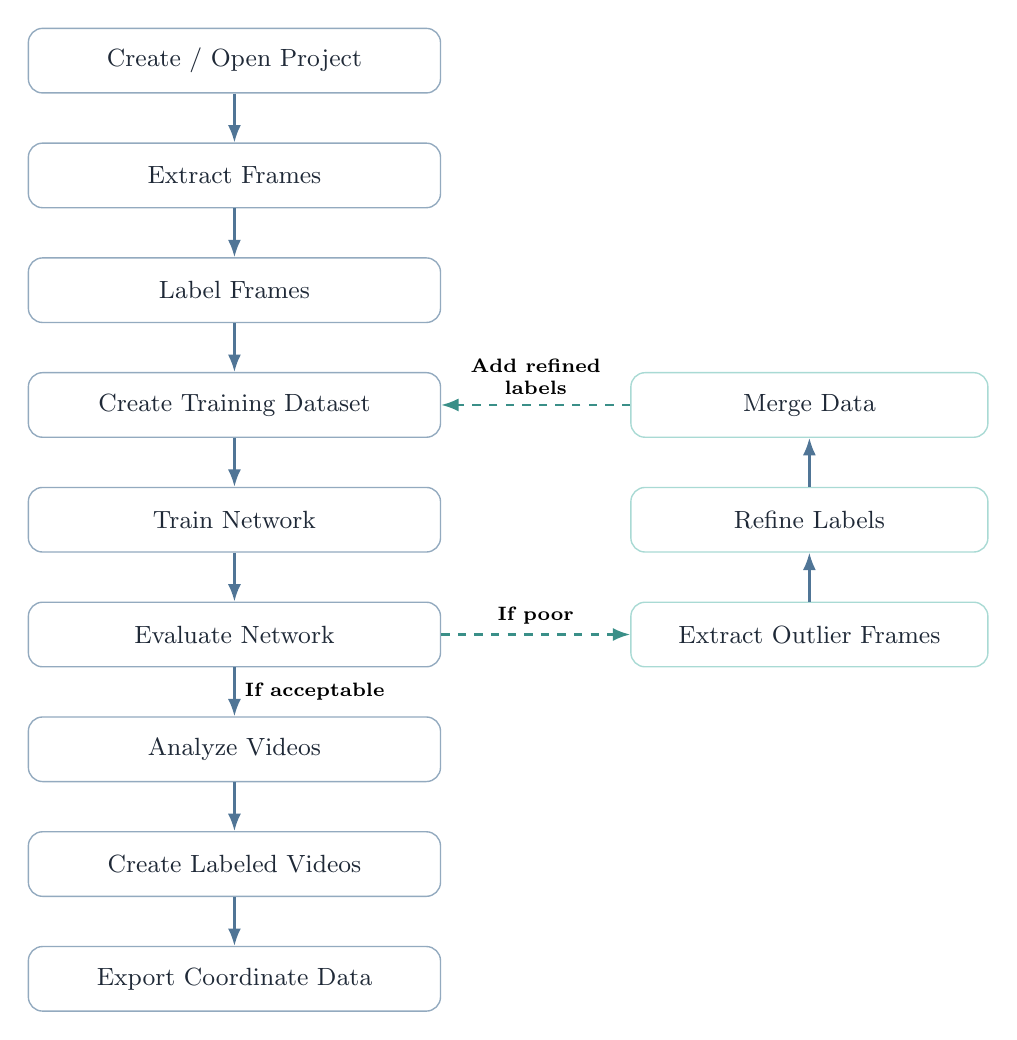
\begin{tikzpicture}[
    node distance=0.62cm,
    box/.style={
        rectangle,
        rounded corners=1.8mm,
        draw=almaBlue!48,
        fill=white,
        text width=5.0cm,
        align=center,
        minimum height=0.82cm,
        font=\small,
        text=almaInk,
        line width=0.5pt
    },
    sidebox/.style={
        rectangle,
        rounded corners=1.8mm,
        draw=diagramTealFrame,
        fill=diagramTealFill,
        text width=4.3cm,
        align=center,
        minimum height=0.82cm,
        font=\small,
        text=almaInk,
        line width=0.5pt
    },
    arrow/.style={
        -{Latex[length=2.2mm]},
        thick,
        draw=almaBlue!78
    },
    dashedarrow/.style={
        -{Latex[length=2.2mm]},
        thick,
        dashed,
        draw=almaTeal!82
    }
]

% Main DLC workflow
\node[box] (open) {Create / Open Project};
\node[box, below=of open] (extract) {Extract Frames};
\node[box, below=of extract] (label) {Label Frames};
\node[box, below=of label] (dataset) {Create Training Dataset};
\node[box, below=of dataset] (train) {Train Network};
\node[box, below=of train] (evaluate) {Evaluate Network};
\node[box, below=of evaluate] (analyze) {Analyze Videos};
\node[box, below=of analyze] (labeled) {Create Labeled Videos};
\node[box, below=of labeled] (export) {Export Coordinate Data};

% Refinement workflow, bottom to top
\node[sidebox, right=2.4cm of evaluate] (outlier) {Extract Outlier Frames};
\node[sidebox, above=of outlier] (refine) {Refine Labels};
\node[sidebox, above=of refine] (merge) {Merge Data};

% Main arrows
\draw[arrow] (open) -- (extract);
\draw[arrow] (extract) -- (label);
\draw[arrow] (label) -- (dataset);
\draw[arrow] (dataset) -- (train);
\draw[arrow] (train) -- (evaluate);
\draw[arrow] (evaluate) -- node[right, font=\scriptsize\bfseries] {If acceptable} (analyze);
\draw[arrow] (analyze) -- (labeled);
\draw[arrow] (labeled) -- (export);

% Refinement branch
\draw[dashedarrow] (evaluate.east) -- node[above, font=\scriptsize\bfseries] {If poor} (outlier.west);

\draw[arrow] (outlier) -- (refine);
\draw[arrow] (refine) -- (merge);

% Return to training dataset creation
\draw[dashedarrow] (merge.west) -- 
node[midway, above, font=\scriptsize\bfseries, align=center] {Add refined\\labels} 
(dataset.east);

\end{tikzpicture}

\end{tcolorbox}
\noindent DeepLabCut provides a labelled hindlimb tracking video, as well as \texttt{x} and \texttt{y} image-coordinate data, and likelihood values for each predicted label. 

% ---------------------------------------------------------
\subsection{Create/Open Project}

A new project can be created selecting the "Create New Project" button. 

\begin{tcolorbox}[
    software settings,
    title=\textbf{Create Project: Recommended Settings}
]
\begin{tabularx}{\linewidth}{KV}
Project & Project name, \texttt{Mouse\_Hindlimb\_Gait}. \\
Experimenter & Enter experimenter name. \\
Location & Select the location for the project to be stored. \\
3D pose estimation project & No\\
Multiple individuals & No\\
Bodyparts to track & Refer to \secref{sec:select-bodyparts}. \\
Files & Input videos for training and testing. \\
Copy videos to project folder & No \\
Select individual files & Enable if selecting individual video files rather than folders. \\
\end{tabularx}
\end{tcolorbox}
An exisiting project can be opened by selecting the \texttt{config.yaml} file from an existing project directory upon clicking "Load Project" button. This file stores the many DeepLabCut settings that can be adjusted accordingly. The \texttt{config.yaml} file is the central project file. If the project is moved to another computer or directory, the paths of \texttt{config.yaml} should be checked before continuing. Upon opening a project, the \textbf{Manage Project} tab will appear:

\begin{tcolorbox}[software settings,title=\textbf{Manage Project: Recommended Settings}]
\begin{tabularx}{\linewidth}{KV}
Active config file & Do not change \\
Engine & PyTorch \\
\end{tabularx}
\end{tcolorbox}


\begin{tcolorbox}[output file box,title=\textbf{Create Project Output Files}]
\begin{tabularx}{\linewidth}{
>{\bfseries\raggedright\arraybackslash}p{0.24\linewidth}|
>{\raggedright\arraybackslash}X
}
\boxedtoprule
Output & Explanation \\
\boxedmidrule
Configuration file & \texttt{config.yaml}\par
The central DeepLabCut project configuration file. It stores the project path, video paths, bodypart labels, training fraction, scorer name, date tag, and analysis settings. \\
Video link or copy & \texttt{[video].mp4}\par
A symlink to the original video when \textbf{Copy videos to project folder} is set to \textbf{No}. If symlink creation fails, DeepLabCut may copy the video instead. \\
Labeled-data folder & \texttt{[video]/}\par
The per-video folder that will store extracted frames and label files. \\
Training-datasets folder & \texttt{training-datasets/}\par
The parent folder for generated training datasets. \\
Model folder & \texttt{dlc-models/}\par
The default model parent folder created with the project. With the PyTorch engine, trained model files are later stored under \texttt{dlc-models-pytorch}. \\
\boxedbottomrule
\end{tabularx}
\end{tcolorbox}


% ---------------------------------------------------------
\subsection{Select Bodyparts}\label{sec:select-bodyparts}

The experimental apparatus is similar to the setup of Zörner et al. (2010), where there are mirrored images from the left, right, and bottom views. As such, the body parts are split into two categories:

\begin{tcolorbox}[blue table box,title=\textbf{Recommended Bodyparts}]
\begin{multicols}{2}
\textbf{Side-view hindlimb bodyparts}
\begin{itemize}
    \item Toe tip
    \item Metatarsophalangeal joint
    \item Ankle
    \item Knee
    \item Hip
    \item Iliac crest
\end{itemize}

\columnbreak

\textbf{Bottom-view bodyparts}
\begin{itemize}
    \item Left hind paw
    \item Right hind paw
    \item Tail base
    \item Body center
\end{itemize}
\end{multicols}
\end{tcolorbox}

These side-view body parts are consistent those used in Aljovic et al. (2022), Zörner et al. (2010), and Weber et al. (2022). DeepLabCut expects each label to correspond to one specific point in the image, so each label should be unique for each view. Strictly follow the proposed ordering when entering body parts labels into DeepLabCut to make Sequential labelling easier in \secref{sec:label-frames}. Same-sided parts should be consecutive to one another. 
\begin{tcolorbox}[
    data callout,
    title=\textbf{Recommended DeepLabCut Bodypart Labels}
]
\begin{multicols}{3}
\textbf{Left side}
\begin{itemize}
    \item \texttt{L\_toe}
    \item \texttt{L\_MTP}
    \item \texttt{L\_ankle}
    \item \texttt{L\_knee}
    \item \texttt{L\_hip}
    \item \texttt{L\_iliac}
\end{itemize}

\columnbreak

\textbf{Right side}
\begin{itemize}
    \item \texttt{R\_toe}
    \item \texttt{R\_MTP}
    \item \texttt{R\_ankle}
    \item \texttt{R\_knee}
    \item \texttt{R\_hip}
    \item \texttt{R\_iliac}
\end{itemize}

\columnbreak

\textbf{Bottom}
\begin{itemize}
    \item \texttt{B\_LHpaw}
    \item \texttt{B\_RHpaw}
    \item \texttt{B\_LFpaw}
    \item \texttt{B\_RFpaw}
    \item \texttt{B\_tailbase}
    \item \texttt{B\_bodycenter}
\end{itemize}
\end{multicols}
\end{tcolorbox}

% ---------------------------------------------------------
\subsection{Extract Frames}

Frames to be manually labelled are extracted from the \textbf{Extract frames} tab. This creates images used for model training.

\begin{tcolorbox}[software settings,title=\textbf{Extract Frames: Recommended Settings}]
\begin{tabularx}{\linewidth}{KV}
Extraction method & automatic \\
Extraction algorithm & kmeans \\
Frame cropping & disabled \\
GUI slider width & 25 \\
Cluster step & 1 \\
Video type & \texttt{mp4} \\
\end{tabularx}
\end{tcolorbox}

\begin{tcolorbox}[output file box,title=\textbf{Extract Frames Output Files}]
\begin{tabularx}{\linewidth}{
>{\bfseries\raggedright\arraybackslash}p{0.24\linewidth}|
>{\raggedright\arraybackslash}X
}
\boxedtoprule
Output & Explanation \\
\boxedmidrule
Extracted frames & \texttt{img[frame].png}\par
Extracted training images selected from the video. The frame number is zero-padded by DeepLabCut, so the exact filename looks like \texttt{img000123.png} or similar depending on video length. Because cropping is disabled, these are full-frame images. \\
\boxedbottomrule
\end{tabularx}
\end{tcolorbox}

Using k-means, extracted frames should automatically select different postures. If the model expects predictions on mice of different experimental conditions, then the videos put into \textbf{Extract frames} should include all experimental conditions. For reference, 450 manually labelled frames were used for hindlimb prediction in Aljovic et al. (2022), and  120 extracted frames were manually labelled (240 total after refinement) in Weber et al. (2022). It should be expected that a range of 240 or more frames would be sufficient to train an acceptable model. 

% ---------------------------------------------------------
\subsection{Label Frames}\label{sec:label-frames}

Manual labeling should be performed through the \textbf{Label frames} tab. Clicking on "Label Frames" opens the napari labeling interface.

\begin{tcolorbox}[software settings,title=\textbf{Napari Interface: Recommended Settings}]
\begin{tabularx}{\linewidth}{KV}
Labelling mode & Sequential \\
Show color scheme & Yes \\
Show trajectories & Yes \\
Show trails & Yes \\
\end{tabularx}
\end{tcolorbox}

In the napari interface, left-clicking when the cursor is the labelling tool places a label. Under sequential labelling mode, the label is automatically switched to the next label (in order) upon placeing down the label. It is also possible to manually select which bodypart label to use by switching the labelling mode \textbf{Sequential} to \textbf{Manual}. Tools that allow for deletion and moving of labels can be switched on the top left of the interface. As a reference guide, a visual representation of body parts can be found here by selecting "Body Parts" and "Joints": 

\begin{tcolorbox}[resource callout]
\url{https://www.imaios.com/en/vet-anatomy/mouse/mouse-whole-body}
\end{tcolorbox}

\underline{\textbf{Ensure that label placement on the body part is correct}}, as incorrect or inconsistent labelling will lead to poor representation of mouse movement that is not shown by error values when evaluating the performance of the model. It is thus important to check all the frames again for correct label placement using the \textbf{Check Labels} button after each session. Skip and do not label body parts that are hidden or outside the frame. Make sure to save the current labels and frames after each session if placed correctly. 

\begin{tcolorbox}[output file box,title=\textbf{Label Frames and Check Labels Output Files}]
\begin{tabularx}{\linewidth}{
>{\bfseries\raggedright\arraybackslash}p{0.24\linewidth}|
>{\raggedright\arraybackslash}X
}
\boxedtoprule
Output & Explanation \\
\boxedmidrule
Saved label table & \texttt{CollectedData\_[scorer].h5}\par
The main saved label file for a video. This is the file DeepLabCut uses when creating the training dataset. \\
Readable label table & \texttt{CollectedData\_[scorer].csv}\par
A human-readable copy of the same label table. It is useful for inspection or manual backup, but the \texttt{.h5} file is the primary training input. \\
Check-label images & \texttt{img[frame]\_bodypart.png}\par
Check-label images generated by the \textbf{Check Labels} tool. These show the manually placed labels overlaid on the extracted frames. \\
\boxedbottomrule
\end{tabularx}
\end{tcolorbox}

% ---------------------------------------------------------
\subsection{Create Training Dataset}

The training dataset is created from the extracted frames using the \textbf{Create training dataset} tab. Weber et al. (2022) uses a 75-25 training to testing data split due to only having 120 frames from their initial frame extraction. The training-testing data split can be edited in \texttt{config.yaml} on \texttt{Line 55}:

\begin{tcolorbox}[
  patch callout,
  left=1mm,
  right=1mm,
  top=1mm,
  bottom=1mm
]
\diffdel{Training Fraction - 0.95}

\vspace{1pt}

\diffadd{Training Fraction - 0.75}
\end{tcolorbox}


With more manually labelled data (150-400 frames), the ratio can be slowly adjusted up to the base split of 95-05. Though with less data (100-150 frames), it is recommended that the split is kept to be around 75-25. 

\begin{tcolorbox}[software settings,title=\textbf{Create Training Dataset: Recommended Settings}]
\begin{tabularx}{\linewidth}{KV}
Shuffle & 1 \\
Network architecture & \texttt{resnet\_50} \\
Weight initialization & Transfer learning - SuperAnimal TopViewMouse \\
Augmentation method & albumentations \\
Overwrite if exists & Unchecked\\
Use existing data split & Unchecked \\
\end{tabularx}
\end{tcolorbox}

\begin{tcolorbox}[output file box,title=\textbf{Create Training Dataset Output Files}]
\begin{tabularx}{\linewidth}{
>{\bfseries\raggedright\arraybackslash}p{0.24\linewidth}|
>{\raggedright\arraybackslash}X
}
\boxedtoprule
Output & Explanation \\
\boxedmidrule
Dataset metadata & \texttt{metadata.yaml}\par
Metadata describing the generated dataset split and shuffle. \\
Merged label dataset & \texttt{CollectedData\_[scorer].h5}\par
The merged label dataset created from all labeled video folders. \\
Readable merged labels & \texttt{CollectedData\_[scorer].csv}\par
A readable copy of the merged label dataset. \\
Training data file & \texttt{Mouse\_Hindlimb\_Gait\_[scorer]75shuffle1.mat}\par
The training data file generated for shuffle 1 using the 75\% training fraction. \\
Split documentation & \texttt{Documentation\_data-Mouse\_Hindlimb\_Gait\_75shuffle1.pickle}\par
The train-test split documentation file for shuffle 1. \\
Training configuration & \texttt{pytorch\_config.yaml}\par
The PyTorch training configuration used by the model. \\
Test pose configuration & \texttt{pose\_cfg.yaml}\par
The test/evaluation pose configuration generated for the shuffle. \\
\boxedbottomrule
\end{tabularx}
\end{tcolorbox}

For an initial model, one shuffle is sufficient. Additional shuffles may be useful later for benchmarking. ResNet-50 is the standard model used in lab environments due to its balanced accuracy and training time. Initalized weights from SuperAnimal TopViewMouse Transfer learning adapts a pretrained top-down view model of mice, allowing for training with little labelled training data. 

% ---------------------------------------------------------
\subsection{Train Network}

The network is trained using the \textbf{Train network} tab after the dataset is created. Nath et al. (2019) suggests at least 100,000 training iterations, while Weber et al. (2022) performed 1,030,000 iterations with loss plateauing at around 100,000 to 300,000 iterations. In Aljovic et al. (2022), the hindlimb model trains 650,000 iterations. We can standardize these iterations to use epochs, where one epoch is one full pass through the training dataset. Therefore, to obtain the number of epochs used:
\[
\text{epochs} =
\left\lceil
\frac{I}
{
\left\lceil 
\frac{f_{\text{train}} \times n}
{B}
\right\rceil
}
\right\rceil
\]

where $I$ is the target iterations, $n$ is the number of manually labeled frames, $B$ is the batch size, and $f_{\text{train}}$ is the training fraction. Note that the default batch size in DeepLabCut is 8, which can be edited in \texttt{config.yaml} at \texttt{Line 61}. It is not documented what batch size and training fraction are used for all papers, thus we assume a batch size of $B=8$ and a training fraction $f_{\text{train}}=0.75$ for epoch approximation: 

 


\begin{tcolorbox}[blue table box,title=\textbf{Training Amounts and Epoch Equivalents}]
\small
\begin{tabularx}{\linewidth}{>{\bfseries}p{0.30\linewidth} p{0.18\linewidth} p{0.18\linewidth} X}
\toprule
Paper & Iterations & Labeled frames & Approx. epochs, $B=8$, $f_{\text{train}}=0.75$ \\
\midrule

Aljovic et al. (2022), hindlimb model 
& 650,000 
& $\sim$450 
& $\sim$15,117 \\

Aljovic et al. (2022), ladder model 
& 400,000 
& $\sim$200 
& $\sim$21,053 \\

Weber et al. (2022) 
& 1,030,000 
& 120 
& $\sim$85,834 \\

\bottomrule
\end{tabularx}
\end{tcolorbox}

Keep in mind that the maximum epochs is an upper bound to the number of epochs used. For small pilot tests, like testing the video quality enhancements of \secref{sec:video-quality-enhancements}, the maximum number of epochs can be set to 200. When conventionally training a high-accuracy model, following a formula: 

\[
\text{epochs} =
\left\lceil
\frac{\text{100,000}}
{
\left\lceil 
\frac{f_{\text{train}} \times n}
{\text{B}}
\right\rceil
}
\right\rceil
\]

Should be a lower bound on the number of epochs used, given that 100,000 is the lower bound on the number of iterations that Nath et al. (2019) suggested for an accurate model. 

\begin{tcolorbox}[software settings,title=\textbf{Train Network: Recommended Settings}]
\begin{tabularx}{\linewidth}{KV}
Shuffle & 1 \\
Display iterations & 5000 \\
Number of snapshots to keep & 3 \\
Maximum epochs & Refer to formulas \\
Save epochs & 500 \\
\end{tabularx}
\end{tcolorbox}

\begin{tcolorbox}[output file box,title=\textbf{Train Network Output Files}]
\begin{tabularx}{\linewidth}{
>{\bfseries\raggedright\arraybackslash}p{0.24\linewidth}|
>{\raggedright\arraybackslash}X
}
\boxedtoprule
Output & Explanation \\
\boxedmidrule
Training log & \texttt{train.txt}\par
The training log file written during PyTorch training. It records configuration and training messages. \\
Training statistics & \texttt{learning\_stats.csv}\par
The training statistics table. This records values such as loss over training epochs. \\
Model snapshots & \texttt{snapshot-[epoch].pt}\par
A saved model snapshot at a scheduled save epoch. With \textbf{Save epochs} set to 500, examples include \texttt{snapshot-500.pt}, \texttt{snapshot-1000.pt}, and later saved checkpoints. \\
Best snapshot & \texttt{snapshot-best-[epoch].pt}\par
The best-snapshot checkpoint, when best-snapshot saving is active for the training run. \\
\boxedbottomrule
\end{tabularx}
\end{tcolorbox}

The training loss will be reported in the Anaconda Prompt (Windows) or Terminal (macOs/Linux) over the iterations, and will decrease over time and eventually begin to plateau. If the loss is still significantly decreasing at the end of training, having more training epochs may improve the model. Conversely, if the loss has plateaued and tracking quality in video analysis is poor, see \secref{sec:dlc-output}. \\
TODO : NINC + Computation Limitations 

% ---------------------------------------------------------
\subsection{Evaluate Network}

The model is evaluated using the \textbf{Evaluate network} tab after training. The evaluation compares model predictions against manually labelled frames. 

\begin{tcolorbox}[software settings,title=\textbf{Evaluate Network: Recommended Settings}]
\begin{tabularx}{\linewidth}{KV}
Shuffle & 1 \\
Compare all bodyparts & Checked \\
Plot predictions & Checked \\
\end{tabularx}
\end{tcolorbox}

\begin{tcolorbox}[output file box,title=\textbf{Evaluate Network Output Files}]
\begin{tabularx}{\linewidth}{
>{\bfseries\raggedright\arraybackslash}p{0.24\linewidth}|
>{\raggedright\arraybackslash}X
}
\boxedtoprule
Output & Explanation \\
\boxedmidrule
Evaluation predictions & \texttt{[DLCscorer].h5}\par
The evaluation prediction table for the selected snapshot. It stores predicted coordinates for the manually labeled train/test frames. \\
Evaluation metrics & \texttt{[DLCscorer]-results.csv}\par
The evaluation metrics for the selected snapshot, including train/test performance values. \\
Combined summary & \texttt{CombinedEvaluation-results.csv}\par
A combined evaluation summary across evaluated snapshots. \\
Training overlay images & \texttt{Training-[video]-img[frame].png}\par
Prediction overlay images for frames assigned to the training set. These are created because \textbf{Plot predictions} is checked. \\
Test overlay images & \texttt{Test-[video]-img[frame].png}\par
Prediction overlay images for frames assigned to the test set. These are created because \textbf{Plot predictions} is checked. \\
Per-keypoint metrics & \texttt{[DLCscorer]-keypoint-results.csv}\par
Optional per-keypoint evaluation file. This is only produced if per-keypoint evaluation is enabled. \\
\boxedbottomrule
\end{tabularx}
\end{tcolorbox}

In the Anaconda Prompt (Windows) or Terminal (macOs/Linux), the evaluation results will return a list of metrics showcasing model performance on the training and testing datasets. For each metric, there exists a reported value for both training and testing. While yielding good results on training generally indicates that the model fits the training set well, it is not indicative of good generalizability. Thus, metrics on test data should be the focal point of evaluation:

\begin{tcolorbox}[blue table box,title=\textbf{DeepLabCut Evaluation Metrics}]
\renewcommand{\arraystretch}{1.25}

\begin{tabularx}{\linewidth}{>{\bfseries}p{3.5cm}X}
\toprule
Metric & Interpretation \\
\midrule

RMSE & Average Euclidean distance between predicted body parts and manually labelled body parts in pixels. Lower values mean the prediction is accurate in placing it near the correct manual label. \\

\midrule

RMSE p-cutoff & RMSE calculated only for predictions above the confidence threshold. This shows the RMSE only of frames that are not low-confidence predictions. \\
\midrule

mAP & Mean average precision. Higher values mean that predicted body parts are likely placed correctly when the model makes a prediction. \\
\midrule

mAR & Mean average recall. Higher values indicate that the model successfully detects the body parts in the image. \\
\bottomrule
\end{tabularx}
\end{tcolorbox}

In general, lower RMSE values and higher mAP/mAR values indicate better model performance. For reference, Weber et al. (2022) reported a runway test RMSE of 5.5 px (0.12 cm), and a Ladder rung test RMSE of 4.7 px (0.14 cm). Nath et al. (2019) states that there should be an expected pixel errors less of less than 5 px for a dataset with 100 labeled frames, and 2.7 px for one with 500 labeled frames. Comparing these measurements, however, aren't standardized to account for image resolution. It is also important to note that these metrics can naturally have variance from human error in manual labelling. 


% ---------------------------------------------------------
\subsection{Extract Outlier Frames and Refine Model (Optional)}

\begin{tcolorbox}[software settings,title=\textbf{Extract Outlier Frames: Recommended Settings}]
\begin{tabularx}{\linewidth}{KV}
Video type & \texttt{mp4} \\
Shuffle & 1 \\
Algorithm & uncertain \\
\end{tabularx}
\end{tcolorbox}

\begin{tcolorbox}[output file box,title=\textbf{Optional Refinement Output Files}]
\begin{tabularx}{\linewidth}{
>{\bfseries\raggedright\arraybackslash}p{0.24\linewidth}|
>{\raggedright\arraybackslash}X
}
\boxedtoprule
Output & Explanation \\
\boxedmidrule
Outlier frames & \texttt{img[frame].png}\par
Newly extracted outlier frames added to the same per-video labeled-data folder. \\
Labeled outlier previews & \texttt{img[frame]labeled.png}\par
Optional labeled outlier-frame preview image, produced only when saving labeled outlier frames is enabled. \\
Machine labels & \texttt{machinelabels-iter0.h5}\par
Machine-predicted labels for the extracted outlier frames at refinement iteration 0. \\
Readable machine labels & \texttt{machinelabels.csv}\par
Readable copy of the current machine-label table. \\
Refined labels & \texttt{MachineLabelsRefine.h5}\par
Refined labels saved after the user manually corrects the machine-labeled outlier frames. \\
\boxedbottomrule
\end{tabularx}
\end{tcolorbox}


% ---------------------------------------------------------
\subsection{Output}\label{sec:dlc-output}

\begin{tcolorbox}[software settings,title=\textbf{Analyze Videos: Recommended Settings}]
\begin{tabularx}{\linewidth}{KV}
Video type & \texttt{mp4} \\
Shuffle & 1 \\
Dynamically crop bodyparts & Unchecked \\
Save result(s) as CSV & Checked \\
Filter predictions & Unchecked \\
Plot trajectories & Checked \\
Show trajectory plots & Checked \\
\end{tabularx}
\end{tcolorbox}

\begin{tcolorbox}[output file box,title=\textbf{Analyze Videos Output Files}]
\begin{tabularx}{\linewidth}{
>{\bfseries\raggedright\arraybackslash}p{0.24\linewidth}|
>{\raggedright\arraybackslash}X
}
\boxedtoprule
Output & Explanation \\
\boxedmidrule
Metadata & \texttt{[video][DLCscorer]\_meta.pickle}\par
Metadata for the analyzed video, including video information and crop settings used during analysis. \\
Full prediction data & \texttt{[video][DLCscorer]\_full.pickle}\par
Full PyTorch prediction data saved before conversion into the standard DeepLabCut dataframe format. \\
Coordinate table & \texttt{[video][DLCscorer].h5}\par
The main DeepLabCut coordinate output. Each frame contains predicted \texttt{x}, \texttt{y}, and likelihood values for each bodypart. \\
Coordinate CSV & \texttt{[video][DLCscorer].csv}\par
A readable CSV copy of the analyzed coordinate output. This is produced because \textbf{Save result(s) as CSV} is checked. \\
Trajectory plot & \texttt{trajectory.png}\par
Bodypart trajectory plot across the video. \\
Coordinate trace plot & \texttt{plot.png}\par
Coordinate trace plot showing position over time. \\
Likelihood trace plot & \texttt{plot-likelihood.png}\par
Likelihood trace plot showing prediction confidence over time. \\
Histogram plot & \texttt{hist.png}\par
Coordinate histogram plot. \\
\boxedbottomrule
\end{tabularx}
\end{tcolorbox}

\begin{tcolorbox}[software settings,title=\textbf{Create Videos: Recommended Settings}]
\begin{tabularx}{\linewidth}{KV}
Video type & \texttt{mp4} \\
Shuffle & 1 \\
Overwrite videos & Disabled \\
Number of trail points & 0 \\
Plot all bodyparts & Checked \\
Draw skeleton & Checked \\
Use filtered data & Unchecked \\
Plotting confidence cutoff & 0.60 \\
Plot trajectories & Checked \\
High quality video & Unchecked \\
\end{tabularx}
\end{tcolorbox}

\begin{tcolorbox}[output file box,title=\textbf{Create Videos Output Files}]
\begin{tabularx}{\linewidth}{
>{\bfseries\raggedright\arraybackslash}p{0.24\linewidth}|
>{\raggedright\arraybackslash}X
}
\boxedtoprule
Output & Explanation \\
\boxedmidrule
Labeled video & \texttt{[video][DLCscorer]\_p60\_labeled.mp4}\par
Labeled video with predicted bodyparts drawn on each frame. The \texttt{p60} suffix comes from the plotting confidence cutoff of 0.60. Because \textbf{Use filtered data} is unchecked, this uses the unfiltered coordinate output. \\
\boxedbottomrule
\end{tabularx}
\end{tcolorbox}


% ---------------------------------------------------------
\section{Data Preprocessing}

The DeepLabCut \texttt{.csv} and \texttt{.h5} output will contain a data point $d_{b, f}$ for every body part $b$ and every frame $f$. The data point $d_{b, f}$ will contain three dimensions:
\[d_{b, f} = \{x_{b, f}, y_{b, f}, p_{b, f}\}\]

\noindent where $x_{b, f}$ is the horizontal coordinate $x$ in pixels from the origin for the body part marker $b$ at frame $f$; $y_{b, f}$ is the vertical coordinate $y$ in pixels from the origin for the body part marker $b$ at frame $f$; and $p_{b, f}$ is the confidence value for the body part marker $b$ at frame $f$. 

\begin{tcolorbox}[
    title=\textbf{DeepLabCut Coordinate Data Structure},
    figure callout
]
\centering
\resizebox{0.92\linewidth}{!}{
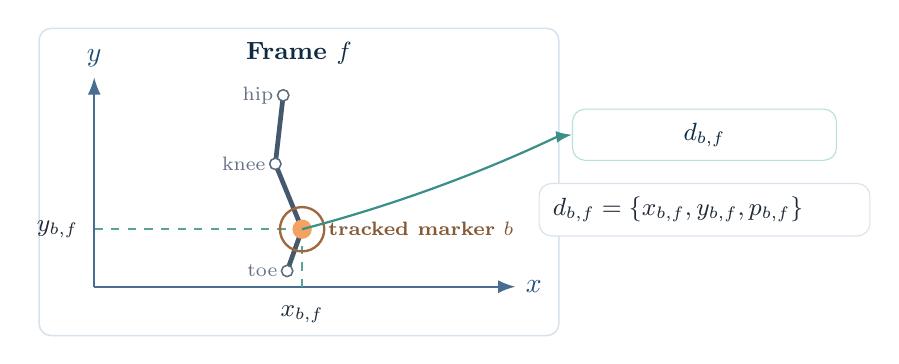
\begin{tikzpicture}[
    axis/.style={-{Latex[length=2.2mm]}, line width=0.75pt, draw=almaBlue!82},
    guide/.style={dashed, line width=0.55pt, draw=almaTeal!68},
    card/.style={rounded corners=1.6mm, draw=almaLine, fill=white, align=left, font=\small, text=almaInk, inner sep=5pt},
    valuecard/.style={rounded corners=1.6mm, draw=diagramTealFrame!85, fill=white, align=center, font=\small, text=almaNavy, inner sep=5pt},
    limb/.style={line width=1.7pt, draw=almaNavy!78, line cap=round, line join=round},
    joint/.style={circle, draw=almaNavy!70, fill=white, line width=0.55pt, inner sep=1.45pt}
]
    \draw[rounded corners=1.5mm, fill=white, draw=almaLine, line width=0.55pt] (0,0) rectangle (6.6,3.9);
    \node[font=\small\bfseries, text=almaNavy] at (3.3,3.58) {Frame $f$};

    \draw[axis] (0.7,0.62) -- (6.05,0.62) node[right, text=almaBlue] {$x$};
    \draw[axis] (0.7,0.62) -- (0.7,3.28) node[above, text=almaBlue] {$y$};

    \coordinate (hip) at (3.1,3.05);
    \coordinate (knee) at (3.0,2.18);
    \coordinate (ankle) at (3.34,1.35);
    \coordinate (toe) at (3.15,0.82);
    \coordinate (marker) at (ankle);

    \draw[limb] (hip) -- (knee) -- (ankle) -- (toe);
    \node[joint] at (hip) {};
    \node[joint] at (knee) {};
    \node[joint] at (toe) {};
    \node[font=\scriptsize, text=almaMuted, anchor=east] at (hip) {hip};
    \node[font=\scriptsize, text=almaMuted, anchor=east] at (knee) {knee};
    \node[font=\scriptsize, text=almaMuted, anchor=east] at (toe) {toe};

    \draw[guide] (marker) -- (3.34,0.62);
    \draw[guide] (marker) -- (0.7,1.35);
    \fill[almaAmber] (marker) circle (3.5pt);
    \draw[almaAmber!65!black, line width=0.85pt] (marker) circle (8pt);
    \node[font=\scriptsize\bfseries, text=almaAmber!55!black, anchor=west] at (3.55,1.35) {tracked marker $b$};
    \node[anchor=north, font=\small, text=almaInk] at (3.34,0.5) {$x_{b,f}$};
    \node[anchor=east, font=\small, text=almaInk] at (0.62,1.35) {$y_{b,f}$};

    \node[valuecard, text width=3.0cm] (data) at (8.45,2.55) {$d_{b,f}$};
    \node[card, text width=3.85cm, below=0.28cm of data] (set) {$d_{b,f}=\{x_{b,f},y_{b,f},p_{b,f}\}$};

    \draw[-{Latex[length=2.0mm]}, thick, draw=almaTeal!82] (marker) .. controls (5.25,1.85) and (6.55,2.52) .. (data.west);
\end{tikzpicture}
}
\end{tcolorbox}

% ---------------------------------------------------------
\subsection{Confidence Threshold}

Data can be filtered through a Python script to discard any data points with a $p_{b, f}$ that is below a confidence threshold. In Weber et al. (2022) the confidence threshold used was $95\%$, with more than $99\%$ of data points passing this range. 

% ---------------------------------------------------------
\subsection{Pixel to Distance Conversion}

The data format is not standardized to account for resolution and distortion. As such,
coordinates are converted from pixels (px) to centimeters (cm)
from the origin. \textbf{Option 1: Manual Calibration Calculation} is a lengthy manual calibration calculation process which identifies any existing camera or mirror distortions in the video. \textbf{Option 2: ALMA Reference Body Segment Calibration} allows for fast and reliable pixel to distance calibration built into the ALMA pipeline, but relies on assumptions of consistent mouse physiology and camera stability. 

% ---------------------------------------------------------
\subsubsection{Option 1: Manual Calibration Calculation}

Calibration should be done with measurement markers in the experimental apparatus that span the entire frame and reflects upon all three mirrors. Only one frame with measurement markers is needed for calibration. A conversion factor $s$ should be calculated for each view $v$ (right side, left side, bottom) in the frame to account for distortions from the mirror. With 3 views, it is expected that 3 conversion factors are calculated for every centimetre. There should also be a conversion factor for vertical and horizontal measurement markers to ensure the camera has no horizontal or vertical stretches.  Moreover, factors should also be calculated for each centimetre location $l$ in the frame to account for parallax error and camera distortions. To calculate the conversion factor from a measurement of 1 centimetre within the video frame from the view $v$, location $l$ and corresponding axis $x$ or $y$:

\[
s_{v, x, l} =
\frac{1\ \text{cm}}
{
|x_2-x_1|
}\text{ }, \text{ } s_{v, y, l} =
\frac{1\ \text{cm}}
{
|y_2-y_1|
}
\]

Where $x_2$ and $x_1$ is the horizontal coordinate ends between the horizontal centimetre measurement in pixels, while $y_2$ and $y_1$ are the vertical coordinate ends of the vertical centimetre measurements in pixels. To determine whether the calibration inconsistency is caused by location, axis, or view, the conversion factors should be compared in stages. First, repeated measurements are compared within the same view and axis to test for location-dependent distortion. Then, the horizontal and vertical axes are compared within the same view. Finally, the right, left, and bottom views are compared.For each view-axis pair, the mean conversion factor across calibration locations is:

\[
\bar{s}_{v,a}
=
\frac{1}{n}
\sum_{l=1}^{n}
s_{v,a,l}
\]


\noindent The location-dependent calibration difference for a given view-axis pair can then be calculated as:

\[
\Delta s_{\mathrm{location}}^{(v,a)}
=
\max_l
\left|
\frac{s_{v,a,l}-\bar{s}_{v,a}}{\bar{s}_{v,a}}
\right|
\times 100
\]

This value takes the worst calibration difference among all centimeters along a view-axis. If \(\Delta s_{\mathrm{location}}^{(v,a)} > \tau\), then the conversion factor changes depending on where the 1 cm marker is measured in the frame. This suggests location-dependent distortion, such as parallax error, perspective distortion, mirror angle distortion, or lens distortion. Accounting for location-specific distortion with conversion factors is difficult, thus it is recommended to recapture videos and adjust the camera setup to fix the issue. If the location check is acceptable, the horizontal and vertical axes can be compared within each view:

\[
\Delta s_{\mathrm{axis}}^{(v)}
=
\left|
\frac{
\bar{s}_{v,\mathrm{x}}-\bar{s}_{v,\mathrm{y}}
}{
\bar{s}_{v,\mathrm{x}}+\bar{s}_{v,\mathrm{y}}
}
\right|
\times 100
\]

If \(\Delta s_{\mathrm{axis}}^{(v)} > \tau\), then the \(x\)- and \(y\)-axis scales differ within the same view. In this case, separate axis-specific conversion factors should be used for that view. If the location and axis checks are acceptable, the views can be compared. The mean conversion factor for each view is:

\[
\bar{s}_{v}
=
\frac{
\bar{s}_{v,\mathrm{x}}+\bar{s}_{v,\mathrm{y}}
}{2}
\]

\noindent The overall mean conversion factor across views is:

\[
\bar{s}_{\mathrm{all}}
=
\frac{
\bar{s}_{\mathrm{right}}+
\bar{s}_{\mathrm{left}}+
\bar{s}_{\mathrm{bottom}}
}{3}
\]

\noindent The view-dependent calibration difference is:

\[
\Delta s_{\mathrm{view}}^{(v)}
=
\left|
\frac{
\bar{s}_{v}-\bar{s}_{\mathrm{all}}
}{
\bar{s}_{\mathrm{all}}
}
\right|
\times 100
\]

If \(\Delta s_{\mathrm{view}}^{(v)} > \tau\), then the right, left, and bottom views do not share the same scale. In this case, separate view-specific conversion factors should be used. The following table details instructions in interpreting the percent difference from the mean conversion factor:

\begin{tcolorbox}[blue table box,title=\textbf{Calibration Consistency Interpretation}]
\small
\renewcommand{\arraystretch}{1.18}

Let the acceptable calibration difference be $\tau = 2\%$

\begin{tabularx}{\linewidth}{
>{\raggedright\arraybackslash\bfseries}p{0.23\linewidth}
>{\raggedright\arraybackslash}p{0.34\linewidth}
>{\raggedright\arraybackslash}X
}
\toprule
Calibration Result & Condition & Scaling Rule \\
\midrule

All checks pass
& $\Delta s_{\mathrm{location}}^{(v,a)} \leq \tau$, 
$\Delta s_{\mathrm{axis}}^{(v)} \leq 2\tau$, and 
$\Delta s_{\mathrm{view}}^{(v)} \leq \tau$
& Use one shared factor: 
$s_{v,\mathrm{x}} = s_{v,\mathrm{y}} = \bar{s}_{\mathrm{all}}$ \\

\midrule

Location-dependent distortion
& $\Delta s_{\mathrm{location}}^{(v,a)} > \tau$ for any view-axis pair
& Recapture videos if possible, or use some sort of complex geometric calibration:
$(X_{\mathrm{cm}},Y_{\mathrm{cm}})=f(x_{\mathrm{px}},y_{\mathrm{px}})$ \\

\midrule

Axis-specific scaling
& $\Delta s_{\mathrm{location}}^{(v,a)} \leq \tau$, but 
$\Delta s_{\mathrm{axis}}^{(v)} > 2\tau$
& Use separate axis factors:
$s_{v,\mathrm{x}}=\bar{s}_{v,\mathrm{x}}$ and
$s_{v,\mathrm{y}}=\bar{s}_{v,\mathrm{y}}$ \\

\midrule

View-specific scaling
& $\Delta s_{\mathrm{location}}^{(v,a)} \leq \tau$, 
$\Delta s_{\mathrm{axis}}^{(v)} \leq 2\tau$, but 
$\Delta s_{\mathrm{view}}^{(v)} > \tau$
& Use one factor per view:
$s_{v,\mathrm{x}} = s_{v,\mathrm{y}} = \bar{s}_{v}$ \\

\midrule

View and axis scaling differ
& $\Delta s_{\mathrm{location}}^{(v,a)} \leq \tau$, but 
$\Delta s_{\mathrm{axis}}^{(v)} > 2\tau$ and 
$\Delta s_{\mathrm{view}}^{(v)} > \tau$
& Use separate view-axis factors:
$s_{v,\mathrm{x}}=\bar{s}_{v,\mathrm{x}}$ and
$s_{v,\mathrm{y}}=\bar{s}_{v,\mathrm{y}}$ \\

\bottomrule
\end{tabularx}
\end{tcolorbox}

\begin{tcolorbox}[
    title=\textbf{Manual Calibration Frame Layout},
    figure callout
]
\centering

\small

\vspace{0.6em}

\resizebox{0.98\linewidth}{!}{%
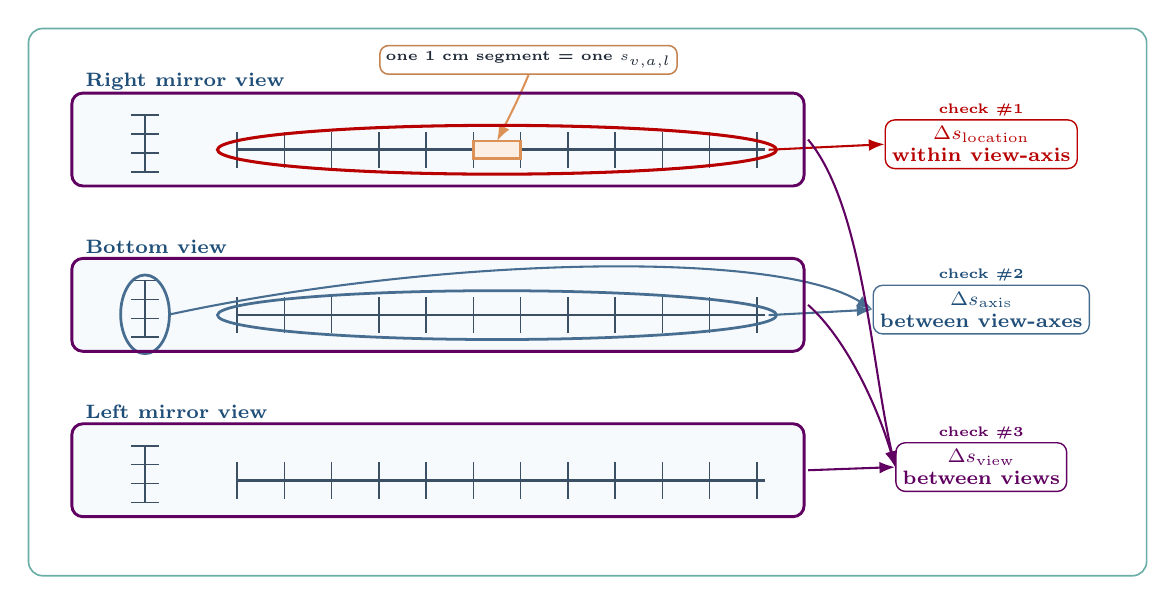
\begin{tikzpicture}[
    view/.style={
        rounded corners=1.4mm,
        draw=almaBlue!45,
        fill=almaMist,
        line width=0.6pt
    },
    ruler/.style={draw=almaNavy!82, line width=0.95pt},
    tick/.style={draw=almaNavy!82, line width=0.55pt},
    label/.style={font=\scriptsize\bfseries, text=almaBlue},
    tag/.style={
        rounded corners=1.2mm,
        draw=calloutFigureFrame,
        fill=white,
        line width=0.5pt,
        align=center,
        font=\scriptsize\bfseries,
        text=almaInk,
        inner sep=2.4pt
    },
    cmnote/.style={
        rounded corners=1.1mm,
        draw=almaAmber!80!black,
        fill=white,
        line width=0.55pt,
        align=center,
        font=\tiny\bfseries,
        text=almaInk,
        inner sep=2.2pt
    },
    order/.style={
        font=\tiny\bfseries,
        text=almaMuted,
        align=center,
        fill=white,
        inner sep=1.0pt
    },
    arrow/.style={-{Latex[length=2.0mm]}, draw=almaTeal!80, line width=0.75pt},
    redfocus/.style={draw=red!72!black, line width=1.1pt},
    bluefocus/.style={draw=almaBlue!82, line width=1.0pt},
    purplefocus/.style={draw=violet!75!black, line width=1.05pt, rounded corners=1.4mm},
    orangefocus/.style={draw=almaAmber!90!black, line width=1.0pt, fill=almaAmber!18}
]

% Outer frame
\draw[rounded corners=1.8mm, draw=calloutFigureFrame, fill=white, line width=0.6pt]
    (0,0) rectangle (14.2,6.95);

% View labels outside boxes
\node[label, anchor=west] at (0.60,6.28) {Right mirror view};
\node[label, anchor=west] at (0.60,4.18) {Bottom view};
\node[label, anchor=west] at (0.60,2.08) {Left mirror view};

% View panels
\foreach \y in {4.95,2.85,0.75} {
    \draw[view] (0.55,\y) rectangle (9.85,\y+1.18);

    % horizontal ruler
    \draw[ruler] (2.65,\y+0.46) -- (9.35,\y+0.46);
    \foreach \x in {2.65,3.25,3.85,4.45,5.05,5.65,6.25,6.85,7.45,8.05,8.65,9.25} {
        \draw[tick] (\x,\y+0.23) -- (\x,\y+0.69);
    }

    % vertical ruler
    \draw[ruler] (1.48,\y+0.18) -- (1.48,\y+0.90);
    \foreach \t in {0.18,0.42,0.66,0.90} {
        \draw[tick] (1.30,\y+\t) -- (1.66,\y+\t);
    }
}

% 1 cm = 1 conversion factor indicator, placed on a middle ruler segment
\draw[orangefocus] (5.65,5.30) rectangle (6.25,5.52);
\node[cmnote, anchor=south] (cmfactor) at (6.35,6.36)
    {one 1 cm segment = one \(s_{v,a,l}\)};
\draw[arrow, draw=almaAmber!90!black] (cmfactor.south) .. controls (6.20,6.00) and (6.05,5.72) .. (5.95,5.52);

% Check 1: Within view-axis
\draw[redfocus] (5.95,5.41) ellipse [x radius=3.55cm, y radius=0.31cm];
\node[tag, draw=red!72!black, text=red!72!black] (loc) at (12.1,5.48)
    {\(\Delta s_{\mathrm{location}}\)\\within view-axis};
\node[order, text=red!72!black, anchor=south] at (loc.north) {check \#1};
\draw[arrow, draw=red!72!black] (9.40,5.41) -- (loc.west);

% Check 2: Between view-axes
\draw[bluefocus] (1.48,3.32) ellipse [x radius=0.31cm, y radius=0.50cm];
\draw[bluefocus] (5.95,3.31) ellipse [x radius=3.55cm, y radius=0.31cm];
\node[tag, draw=almaBlue!82, text=almaBlue] (axis) at (12.1,3.38)
    {\(\Delta s_{\mathrm{axis}}\)\\between view-axes};
\node[order, text=almaBlue, anchor=south] at (axis.north) {check \#2};
\draw[arrow, draw=almaBlue!82] (9.40,3.31) -- (axis.west);
\draw[arrow, draw=almaBlue!82] (1.80,3.32) .. controls (5.2,4.05) and (9.5,4.15) .. (axis.west);

% Check 3: Between views
\draw[purplefocus] (0.55,4.95) rectangle (9.85,6.13);
\draw[purplefocus] (0.55,2.85) rectangle (9.85,4.03);
\draw[purplefocus] (0.55,0.75) rectangle (9.85,1.93);

\node[tag, draw=violet!75!black, text=violet!75!black] (viewcheck) at (12.1,1.38)
    {\(\Delta s_{\mathrm{view}}\)\\between views};
\node[order, text=violet!75!black, anchor=south] at (viewcheck.north) {check \#3};

\draw[arrow, draw=violet!75!black] (9.90,5.54) .. controls (10.6,4.7) and (10.7,2.7) .. (viewcheck.west);
\draw[arrow, draw=violet!75!black] (9.90,3.44) .. controls (10.4,3.0) and (10.8,2.1) .. (viewcheck.west);
\draw[arrow, draw=violet!75!black] (9.90,1.34) -- (viewcheck.west);

\end{tikzpicture}
}

\end{tcolorbox}




Location-dependent distortion should be checked first because if scale changes across the frame, view-specific or axis-specific conversion factors will not be reliable. Apply the conversion factor using a script. Each bodypart coordinate should be assigned to its corresponding view before conversion. Let \(B_v\) denote the set of bodyparts measured in view \(v\). For every datapoint \(d_{b,f}\) where \(b \in B_v\), the conversion factors \(s_{v,\mathrm{x}}\) and \(s_{v,\mathrm{y}}\) should be used:

\[
d_{b,f}^{\mathrm{cm}}
=
\left(
s_{v,\mathrm{x}} x_{b,f},
\;
s_{v,\mathrm{y}} y_{b,f}, \; p_{b, f}
\right)
\]

% ---------------------------------------------------------
\subsubsection{Option 2: ALMA Reference Body Segment Calibration}

In the ALMA pipeline, pixel to centimetre calibration is automated by referencing the known distance between mouse body parts. In the ALMA interface, select \textbf{Reference Body Segment (Recommended)}, and select the reference segment that is most visible throughout the labelled video: \texttt{ankle\_toe, hip\_knee, knee\_ankle, ankle\_mtp}. Segment length must be measured directly from the mouse, which must be provided in the setting \textbf{Segment Length (cm)}. This assumes consistent body part size ratios in the mice. Measurements may need to be performed on each mouse. It is important to note that ALMA does not convert pixels to cm for its calculations for 12 of its variability parameters. 

% ---------------------------------------------------------
\subsection{Coordinate Inversion}\label{sec:coordinate-inversion}

Some mirror views may be vertically inverted. Since body part markers are only compared in respect to other body parts of the same view during gait analysis, inverting the point in respect to the entire frame does not change the relationship between data points of the same view. As such, the coordinate can be corrected by:

\[
y' = H - y
\]

\noindent where \(H\) is the height of the full image. Let \(B_v\) denote the set of bodyparts measured in view \(v\). For every datapoint \(d_{b,f}\) where \(b \in B_v\), belonging to a vertically inverted view \(v\), the corrected pixel coordinate should be:

\[
d_{b,f}' =
(x_{b,f}, \; H - y_{b,f}, \; p_{b, f})
\]

% =========================================================
\section{ALMA Installation and Setup}

\subsection{Download the ALMA Repository}

The official ALMA repository can be found at:

\begin{tcolorbox}[resource callout]
\url{https://github.com/sollan/alma}
\end{tcolorbox}

\noindent Open \textbf{Anaconda Prompt} on Windows, or \textbf{Terminal} on macOS/Linux. Navigate to the Downloads folder.
\\
\noindent On Windows:

\begin{tcolorbox}[command callout]
\begin{verbatim}
cd %USERPROFILE%\Downloads
\end{verbatim}
\end{tcolorbox}

\noindent If the Downloads folder is on the D: drive, use:

\begin{tcolorbox}[command callout]
\begin{verbatim}
cd /d D:\Downloads
\end{verbatim}
\end{tcolorbox}

\noindent On macOS or Linux, use:

\begin{tcolorbox}[command callout]
\begin{verbatim}
cd ~/Downloads
\end{verbatim}
\end{tcolorbox}

\noindent Then clone the ALMA repository:

\begin{tcolorbox}[command callout]
\begin{verbatim}
git clone https://github.com/sollan/alma.git
\end{verbatim}
\end{tcolorbox}

\subsection{Navigate to the ALMA Folder}

After cloning the repository, navigate into the ALMA folder:

\begin{tcolorbox}[command callout]
\begin{verbatim}
cd alma
\end{verbatim}
\end{tcolorbox}

\subsection{Create the ALMA Environment}

Run the following command from inside the ALMA folder:

\begin{tcolorbox}[command callout]
\begin{verbatim}
conda env create -f conda_env_python_3_10.yml
\end{verbatim}
\end{tcolorbox}

\subsection{Activate the ALMA Environment}

From the same Anaconda Prompt or Terminal, activate the ALMA environment:

\begin{tcolorbox}[command callout]
\begin{verbatim}
conda activate venv_python_3_10
\end{verbatim}
\end{tcolorbox}

\subsection{Launch ALMA}

On the very same terminal where the environment was activated, launch ALMA with:

\begin{tcolorbox}[command callout]
\begin{verbatim}
python ./alma.py
\end{verbatim}
\end{tcolorbox}

\noindent Ensure that the ALMA interface opens. The environment must be activated before every launch of ALMA. 

% ---------------------------------------------------------
\section{ALMA Side-view Gait Parameter Analysis}

From the main menu, select \textbf{"Open"} under \textbf{"Gait Kinematics"}, then select \textbf{"Bulk analysis"}. From the file directory, select the folder \texttt{\textbackslash{}videos} within the DeepLabCut project folder. Two iterations should be performed on ALMA, one for the left side view of the mouse and one for the right side view of the mouse. Each iteration outputs 44 parameters, totalling 88 parameters. 

% ---------------------------------------------------------
\subsection{Confirm Body Part Mapping}

For the left and right iterations of the ALMA process, match the following ALMA body parts to the .csv body parts:

\begin{tcolorbox}[
    mapping settings,
    title=\textbf{ALMA Bodypart Mapping: Left and Right Side}
]
\begin{tabularx}{\linewidth}{
>{\bfseries\color{almaNavy}\raggedright\arraybackslash}p{0.27\linewidth}
>{\raggedright\arraybackslash}p{0.30\linewidth}
>{\raggedright\arraybackslash}X
}
\toprule
\textbf{ALMA Bodypart} & \textbf{Left Side Label} & \textbf{Right Side Label} \\
\midrule
toe & \texttt{L\_toe} & \texttt{R\_toe} \\
MTP & \texttt{L\_MTP} & \texttt{R\_MTP} \\
ankle & \texttt{L\_ankle} & \texttt{R\_ankle} \\
knee & \texttt{L\_knee} & \texttt{R\_knee} \\
hip & \texttt{L\_hip} & \texttt{R\_hip} \\
iliac crest & \texttt{L\_iliac} & \texttt{R\_iliac} \\
\bottomrule
\end{tabularx}
\end{tcolorbox}

\noindent Select \textbf{Confirm Mapping} after completing the mapping for each side.




% ---------------------------------------------------------
\subsection{Configure Analysis Settings}

In the analysis settings, configure it to be:
\begin{tcolorbox}[
    software settings,
    title=\textbf{ALMA Kinematic Analysis: Recommended Settings}
]

\begin{tabularx}{\linewidth}{KV}
\textbf{Recording mode} & Spontaneous walking \\

\textbf{Spatial calibration method} & Manual Pixel-to-CM Ratio \\

\textbf{Pixels per CM} & 1.00 \\

\textbf{Walking direction} & Auto-detect \\

\textbf{Drag clearance threshold} & 0.10 cm \\

\textbf{Drag detection sensitivity} & 4 frames \\

\textbf{Low-pass filter cutoff} & 6.0 Hz \\

\textbf{Step height range} & 0.00--5.00 cm \\

\textbf{Stride length range} & 0.00--20.00 cm \\
\end{tabularx}

\end{tcolorbox}

\noindent The pixel calibration is set to 1.00 since the calibration is already performed during data pre-processing. The step and stride lengths are put to the maximum since filtering the data an additional time would require extra standardization steps when extracting non-ALMA parameters. Once these settings are selected, in the \textbf{"Select Output \& Run Analysis"} window, select the output folder to be the \texttt{\textbackslash{}Output} in the ALMA directory, and click \textbf{"Start Analysis"}.

% ---------------------------------------------------------
\subsection{ALMA Output}

\begin{tcolorbox}[output file box,title=\textbf{ALMA Spontaneous Walking Output Files}]
\begin{tabularx}{\linewidth}{
>{\bfseries\raggedright\arraybackslash}p{0.24\linewidth}|
>{\raggedright\arraybackslash}X
}
\boxedtoprule
Output & Explanation \\
\boxedmidrule

Parameter table &
\texttt{[video]\_parameters.csv}

The main ALMA spontaneous-walking gait output. Each row represents one detected
gait cycle, with the extracted kinematic parameters for that cycle. \\

Coordinate table &
\texttt{[video]\_coordinates.csv}

The processed coordinate output used for gait analysis. This contains ALMA's pre-processed and filtered data. \\

Stickplot figure &
\texttt{[video]\_stickplot.svg}

A visual summary of the continuous detected strides. This is useful
for checking whether the detected stride pattern is acceptable. \\

\boxedbottomrule
\end{tabularx}
\end{tcolorbox}


ALMA outputs 44 kinematic parameters:

\begin{tcolorbox}[parameter table box,title=\textbf{ALMA Parameter List}]
\begin{tabularx}{\linewidth}{>{\raggedright\arraybackslash}p{0.045\linewidth}
                  |>{\raggedright\arraybackslash}p{0.30\linewidth}
                  |>{\raggedright\arraybackslash}X
                  |>{\centering\arraybackslash}p{0.06\linewidth}}
\boxedtoprule
\textbf{\#} & \textbf{Parameter Name} & \textbf{ALMA .csv Output Parameter Name} & \textbf{Units} \\
\boxedmidrule

1 & Cycle duration & \texttt{cycle duration (s)} & s \\
2 & Cycle duration & \texttt{cycle duration (no. frames)} & frames \\
3 & Cycle velocity & \texttt{cycle velocity (cm/s)} & cm/s \\
4 & Stride length & \texttt{stride length (cm)} & cm \\
5 & Stance duration & \texttt{stance duration (s)} & s \\
6 & Swing duration & \texttt{swing duration (s)} & s \\
7 & Swing percentage & \texttt{swing percentage (\%)} & \% \\
8 & Stance percentage & \texttt{stance percentage (\%)} & \% \\
9 & Mean toe-to-crest distance & \texttt{mean toe-to-crest distance (cm)} & cm \\
10 & Maximum toe-to-crest distance & \texttt{max toe-to-crest distance (cm)} & cm \\
11 & Minimum toe-to-crest distance & \texttt{min toe-to-crest distance (cm)} & cm \\
12 & Toe-to-crest distance SD & \texttt{toe-to-crest distance SD (cm)} & cm \\
13 & Step height & \texttt{step height (cm)} & cm \\
14 & Maximum swing velocity & \texttt{max velocity during swing (cm/s)} & cm/s \\
15 & MTP joint extension & \texttt{mtp joint extension (deg)} & deg \\
16 & MTP joint flexion & \texttt{mtp joint flexion (deg)} & deg \\
17 & MTP joint amplitude & \texttt{mtp joint amplitude (deg)} & deg \\
18 & MTP joint SD & \texttt{mtp joint SD (deg)} & deg \\
19 & Ankle joint extension & \texttt{ankle joint extension (deg)} & deg \\
20 & Ankle joint flexion & \texttt{ankle joint flexion (deg)} & deg \\
21 & Ankle joint amplitude & \texttt{ankle joint amplitude (deg)} & deg \\
22 & Ankle joint SD & \texttt{ankle joint SD (deg)} & deg \\
23 & Knee joint extension & \texttt{knee joint extension (deg)} & deg \\
24 & Knee joint flexion & \texttt{knee joint flexion (deg)} & deg \\
25 & Knee joint amplitude & \texttt{knee joint amplitude (deg)} & deg \\
26 & Knee joint SD & \texttt{knee joint SD (deg)} & deg \\
27 & Hip joint extension & \texttt{hip joint extension (deg)} & deg \\
28 & Hip joint flexion & \texttt{hip joint flexion (deg)} & deg \\
29 & Hip joint amplitude & \texttt{hip joint amplitude (deg)} & deg \\
30 & Hip joint SD & \texttt{hip joint SD (deg)} & deg \\
31 & Drag duration & \texttt{drag duration (s)} & s \\
32 & Drag percentage & \texttt{drag percentage (\%)} & \% \\
33 & Variability x, 5 strides, mean & \texttt{Variability x plane 5 strides mean} & cm \\
34 & Variability x, 5 strides, SD & \texttt{Variability x plane 5 strides SD} & cm \\
35 & Variability y, 5 strides, mean & \texttt{Variability y plane 5 strides mean} & cm \\
36 & Variability y, 5 strides, SD & \texttt{Variability y plane 5 strides SD} & cm \\
37 & Variability xy, 5 strides, mean & \texttt{Variability xy plane 5 strides mean} & cm \\
38 & Variability xy, 5 strides, SD & \texttt{Variability xy plane 5 strides SD} & cm \\
39 & Variability x, 10 strides, mean & \texttt{Variability x plane 10 strides mean} & cm \\
40 & Variability x, 10 strides, SD & \texttt{Variability x plane 10 strides SD} & cm \\
41 & Variability y, 10 strides, mean & \texttt{Variability y plane 10 strides mean} & cm \\
42 & Variability y, 10 strides, SD & \texttt{Variability y plane 10 strides SD} & cm \\
43 & Variability xy, 10 strides, mean & \texttt{Variability xy plane 10 strides mean} & cm \\
44 & Variability xy, 10 strides, SD & \texttt{Variability xy plane 10 strides SD} & cm \\


\boxedbottomrule
\end{tabularx}
\end{tcolorbox}

% ---------------------------------------------------------
\section{Additional Post-ALMA Parameters}

The 88 extracted ALMA hind limb parameters may not account for all relevant features in mouse gait analysis. ALMA only extracts the side-view gait parameters, missing important gait features observable from different views. To address this limitation, the existing 88 ALMA parameters are merged with 30 non-overlapping parameters from the RustLab1 Gait Analysis scripts from Weber et al. (2022), and 14 additional gait parameters created with original scripts; totalling 132 gait parameters. To prevent overfitting, it is recommended to have a moderately large number set of markerless tracking data. Smoothing and gait cycle detection must be performed on non-ALMA scripts to standardize features.

\begin{tcolorbox}[output file box,title=\textbf{Stroke Pilot Implementation}]
The application now uses the synchronized Bottom view as the authoritative
bilateral event source. A canonical cycle begins at a left-hindpaw stance onset
and ends immediately before the next left-hindpaw stance onset; the right
hindpaw onset is paired inside that frame interval. The identical source-frame
window is then applied to the Left and Middle (Right-role) side views. The
legacy per-view ALMA files are retained, but the scientific combined table is
not joined by row position.

The pilot implements six of the 14 custom features: mean and variance of
hindlimb base of support, left and right paw-to-midline distance, bilateral
phase offset, and bilateral stance overlap. It also derives six signed
contralesional-versus-ipsilesional asymmetry indices. The eight MTP/knee-height
custom features and forelimb retraining are deferred. Consequently, this pilot
is a hindlimb-focused longitudinal analysis rather than a complete
forelimb-inclusive reproduction of Weber et al.
\end{tcolorbox}

\begin{tcolorbox}[
    figure callout,
    title=\textbf{Gait Parameter Extraction Pipeline}
]

\centering
\resizebox{0.95\linewidth}{!}{
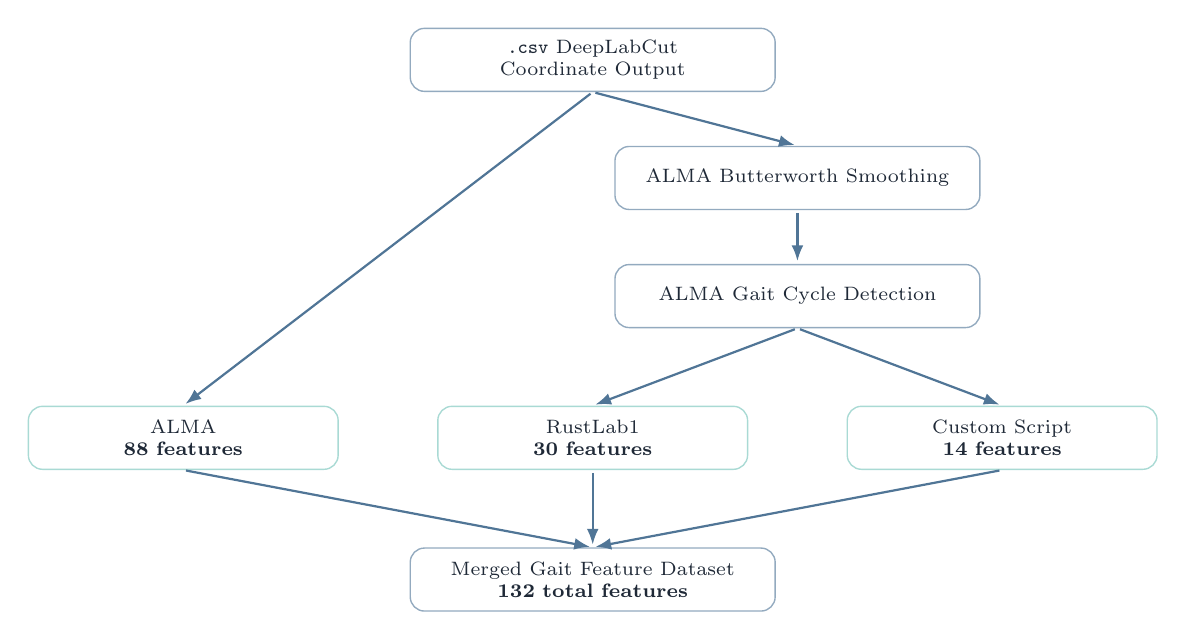
\begin{tikzpicture}[
    box/.style={
        rectangle,
        rounded corners=1.8mm,
        draw=diagramTealFrame,
        fill=diagramTealFill,
        text width=3.7cm,
        align=center,
        minimum height=0.8cm,
        font=\scriptsize,
        text=almaInk,
        line width=0.5pt
    },
    mainbox/.style={
        rectangle,
        rounded corners=1.8mm,
        draw=almaBlue!48,
        fill=white,
        text width=4.4cm,
        align=center,
        minimum height=0.8cm,
        font=\scriptsize,
        text=almaInk,
        line width=0.5pt
    },
    arrow/.style={
        -{Latex[length=2.0mm]},
        thick,
        draw=almaBlue!78,
        shorten >=1pt,
        shorten <=1pt
    }
]

% Nodes
\node[mainbox] (dlc) at (0,0) {
\texttt{.csv} DeepLabCut\\
Coordinate Output
};

\node[mainbox] (cycle) at (2.6,-1.5) {
ALMA Butterworth Smoothing
};

\node[mainbox] (smooth) at (2.6,-3.0) {
ALMA Gait Cycle Detection
};

% Feature extraction nodes on same horizontal line
\node[box] (alma) at (-5.2,-4.8) {
ALMA\\
\textbf{88 features}
};

\node[box] (rustlab) at (0,-4.8) {
RustLab1\\
\textbf{30 features}
};

\node[box] (custom) at (5.2,-4.8) {
Custom Script\\
\textbf{14 features}
};

% Merged output
\node[mainbox] (merged) at (0,-6.6) {
Merged Gait Feature Dataset\\
\textbf{132 total features}
};

% Arrows from middle of boxes
\draw[arrow] (dlc.south) -- (alma.north);
\draw[arrow] (dlc.south) -- (cycle.north);

\draw[arrow] (cycle.south) -- (smooth.north);

\draw[arrow] (smooth.south) -- (rustlab.north);
\draw[arrow] (smooth.south) -- (custom.north);

\draw[arrow] (alma.south) -- (merged.north);
\draw[arrow] (rustlab.south) -- (merged.north);
\draw[arrow] (custom.south) -- (merged.north);

\end{tikzpicture}
}

\end{tcolorbox}

% ---------------------------------------------------------
\subsection{ALMA Butterworth Low-pass Filter}

ALMA smooths marker coordinate trajectories using a fifth-order Butterworth
low-pass filter. To standardize RustLab1 and custom scripts with ALMA, the same
filter should be applied to all marker coordinates before parameter extraction. Given a video frame rate \(F\) and cutoff
frequency \(f_c\), the normalized cutoff frequency $W_n$ is:

\[
W_n = \frac{f_c}{F/2}
\]

\noindent In this case, ALMA uses a cutoff is $f_c = 6\,\mathrm{Hz}$. ALMA also uses a fifth-order Butterworth low-pass filter. As such, the filtered coordinates obtained by zero-phase forward-backward filtering are:
\[
{x'}_{b,f}
=
\mathrm{filtfilt}
\left(
\text{Butterworth}_5(W_n), \;
x_{b,f}
\right)
\]

\[
{y'}_{b,f}
=
\mathrm{filtfilt}
\left(
\text{Butterworth}_5(W_n), \;
y_{b,f}
\right)
\]


\noindent The filtered data point is thus:

\[
{d'}_{b,f}
=
\{\tilde{x}_{b,f}, \tilde{y}_{b,f}, p_{b,f}\}.
\]


% ---------------------------------------------------------
\subsection{ALMA Gait Cycle Standardization}

ALMA's spontaneous walking gait analysis defines a gait cycle $i$ as the interval from stance onset of one toe
to the next stance onset of the same toe:

\[
\mathrm{c}_{i}
=
\left[
f_{\mathrm{stance},i},
f_{\mathrm{stance},i+1} - 1
\right],
\]

\noindent where \(f_{\mathrm{stance},i}\) is the stance onset
frame for cycle \(i\), and \(f_{\mathrm{stance},i+1}\) is the stance
onset for the next cycle $i+1$ of the same toe. A frame is only classified as stance if its toe's $x$ coordinate is close to unchanged. The change in $x$ at frame $f$, $\Delta x_f$ can be defined as:

\[
\Delta{x_f} = |x_{f} - x_{f-1}|
\]

\noindent whereas a stance frame onset for its new cycle $i$ is then:

\[
\Delta{x_f} <= 0.001 \to f_{\text{stance, i}}
\]

\noindent To ensure correctness, the change in $x$ coordinate position between two consecutive stances must be greater than 20 pixels. A comparison is made with the previous cycle $i-1$. All stance frames thus must also satisfy the condition:

\[
|x_{f_{\text{stance}, i}}-x_{f_{\text{stance}, i-1}}| > 20 \to f_{\text{stance}, i}
\]

\noindent Frames that do not satisfy both conditions will not be classified as a stance onset frame.

\subsection{RustLab1 Gait Analysis Outputs}

There are a total of 106 gait parameters used in the Weber et al. (2022) DeepLabCut Gait analysis. The script to extract them can be found in RustLab1's public repository:  

\begin{tcolorbox}[resource callout]
\url{https://github.com/rustlab1/DLC-Gait-Analysis/tree/main}
\end{tcolorbox}

\noindent Only 30 of the 106 gait parameters extracted by the scripts are both hind-limb specific and non-overlapping with the 44 parameters from ALMA. After splitting the DeepLabCut data into the same gait cycles as ALMA, the 106 parameters can be extracted through the RustLab1 script. Then, the dataset is filtered to the 30 relevant parameters, and merged back with the ALMA gait parameter data set. The 30 relevant parameters are as follows:

\begin{tcolorbox}[parameter table box,title=\textbf{RustLab1 Parameter List}]
\begin{tabularx}{\linewidth}{>{\raggedright\arraybackslash}p{0.045\linewidth}
                  |>{\raggedright\arraybackslash}p{0.36\linewidth}
                  |>{\raggedright\arraybackslash}X
                  |>{\centering\arraybackslash}p{0.06\linewidth}}
\boxedtoprule
\textbf{\#} & \textbf{Parameter Name} & \textbf{RustLab1 .csv Output Parameter Name} & \textbf{Units} \\
\boxedmidrule

1  & Left hindpaw mean angle & \texttt{LB\_\_avg\_Angle} & deg \\
2  & Left hindpaw maximum angle & \texttt{LB\_\_max\_Angle} & deg \\
3  & Left hindpaw minimum angle & \texttt{LB\_\_min\_Angle} & deg \\
4  & Right hindpaw mean angle & \texttt{RB\_\_avg\_Angle} & deg \\
5  & Right hindpaw maximum angle & \texttt{RB\_\_max\_Angle} & deg \\
6  & Right hindpaw minimum angle & \texttt{RB\_\_min\_Angle} & deg \\

7  & Left ankle average height & \texttt{l-back-ankle\_\_Average\_Height} & mm \\
8  & Left ankle vertical excursion & \texttt{l-back-ankle\_\_Movement} & mm \\
9  & Left hindpaw average height & \texttt{l-back-toe\_\_Average\_Height} & mm \\
10 & Left hip average height & \texttt{l-hip\_\_Average\_Height} & mm \\
11 & Left hip vertical excursion & \texttt{l-hip\_\_Movement} & mm \\
12 & Left iliac crest average height & \texttt{l-iliac-crest\_\_Average\_Height} & mm \\
13 & Left iliac crest vertical excursion & \texttt{l-iliac-crest\_\_Movement} & mm \\

14 & Right ankle average height & \texttt{r-back-ankle\_\_Average\_Height} & mm \\
15 & Right ankle vertical excursion & \texttt{r-back-ankle\_\_Movement} & mm \\
16 & Right hindpaw average height & \texttt{r-back-toe\_\_Average\_Height} & mm \\
17 & Right hip average height & \texttt{r-hip\_\_Average\_Height} & mm \\
18 & Right hip vertical excursion & \texttt{r-hip\_\_Movement} & mm \\
19 & Right iliac crest average height & \texttt{r-iliac-crest\_\_Average\_Height} & mm \\
20 & Right iliac crest vertical excursion & \texttt{r-iliac-crest\_\_Movement} & mm \\

21 & Left hindpaw average position relative to hip & \texttt{left\_\_back\_\_average} & mm \\
22 & Left hindpaw median position relative to hip & \texttt{left\_\_back\_\_median} & mm \\
23 & Left hindpaw protraction relative to hip & \texttt{left\_\_back\_\_protraction} & mm \\
24 & Left hindpaw retraction relative to hip & \texttt{left\_\_back\_\_retraction} & mm \\
25 & Right hindpaw average position relative to hip & \texttt{right\_\_back\_\_average} & mm \\
26 & Right hindpaw median position relative to hip & \texttt{right\_\_back\_\_median} & mm \\
27 & Right hindpaw protraction relative to hip & \texttt{right\_\_back\_\_protraction} & mm \\
28 & Right hindpaw retraction relative to hip & \texttt{right\_\_back\_\_retraction} & mm \\

29 & Left hip displacement per step & \texttt{left\_\_back\_\_movement\_per\_step} & cm \\
30 & Right hip displacement per step & \texttt{right\_\_back\_\_movement\_per\_step} & cm \\
\boxedbottomrule
\end{tabularx}
\end{tcolorbox}

% ---------------------------------------------------------
\subsection{Parameters Requiring New Scripts (Optional)}


\begin{tcolorbox}[parameter table box,title=\textbf{Custom Parameter List}]
\begin{tabularx}{\linewidth}{>{\raggedright\arraybackslash}p{0.045\linewidth}
                  |>{\raggedright\arraybackslash}p{0.36\linewidth}
                  |>{\raggedright\arraybackslash}X
                  |>{\centering\arraybackslash}p{0.06\linewidth}}
\boxedtoprule
\textbf{\#} & \textbf{Parameter Name} & \textbf{Custom .csv Output Parameter} & \textbf{Units} \\
\boxedmidrule

1 & Mean hindlimb base of support & \texttt{mean\_hindlimb\_base\_support} & cm \\
2 & Variance hindlimb base of support & \texttt{variance\_hindlimb\_base\_support} & cm\textsuperscript{2} \\
3 & Left hindpaw midline distance & \texttt{left\_hindpaw\_midline\_distance} & cm \\
4 & Right hindpaw midline distance & \texttt{right\_hindpaw\_midline\_distance} & cm \\
5 & Left--right hindlimb phase offset & \texttt{left\_right\_hindlimb\_phase\_offset} & \% \\
6 & Hindlimb stance overlap fraction & \texttt{hindlimb\_stance\_overlap\_fraction} & \% \\

7 & Left MTP average height & \texttt{left\_mtp\_average\_height} & cm \\
8 & Left MTP vertical excursion & \texttt{left\_mtp\_vertical\_excursion} & cm \\
9 & Right MTP average height & \texttt{right\_mtp\_average\_height} & cm \\
10 & Right MTP vertical excursion & \texttt{right\_mtp\_vertical\_excursion} & cm \\

11 & Left knee average height & \texttt{left\_knee\_average\_height} & cm \\
12 & Left knee vertical excursion & \texttt{left\_knee\_vertical\_excursion} & cm \\
13 & Right knee average height & \texttt{right\_knee\_average\_height} & cm \\
14 & Right knee vertical excursion & \texttt{right\_knee\_vertical\_excursion} & cm \\

\boxedbottomrule
\end{tabularx}
\end{tcolorbox}
 

Let the superscripts \(L\) and \(R\) denote the left and right hindlimbs.
Let \(c_i\) denote gait cycle \(i\), and let \(a_i\) denote the stance interval
within that gait cycle. The number of frames in an interval is denoted using
vertical bars, such as \(|c_i^L|\), \(|a_i^L|\), or
\(|a_i^L \cap a_i^R|\). Let \(h_{b,f}\) denote the calibrated vertical height,
in cm, of body part \(b\) at frame \(f\). Each result below is calculated for
one gait cycle \(i\).

\begin{tcolorbox}[compact table box,title=\textbf{Custom Parameter Calculations}]
\tiny
\setlength{\tabcolsep}{2pt}
\renewcommand{\arraystretch}{0.9}

\newcommand{\TinyCalcEq}[1]{%
{\fontsize{6.6pt}{7.2pt}\selectfont
\(\displaystyle #1\)}%
}

\begin{tabularx}{\linewidth}{
>{\bfseries\raggedright\arraybackslash}p{0.045\linewidth}|
>{\bfseries\raggedright\arraybackslash}p{0.23\linewidth}|
>{\raggedright\arraybackslash}X
}
\boxedtoprule
\# & Parameter & Calculation \\
\boxedmidrule

1 & Mean hindlimb base of support &
\TinyCalcEq{
\text{\texttt{mean\_hindlimb\_base\_support}}_{i}
=
\frac{
\sum_{f \in a_i^{L} \cap a_i^{R}}
\sqrt{
\left(x_{\mathrm{hindpaw},f}^{L} - x_{\mathrm{hindpaw},f}^{R}\right)^2
+
\left(y_{\mathrm{hindpaw},f}^{L} - y_{\mathrm{hindpaw},f}^{R}\right)^2
}
}{
|a_i^{L} \cap a_i^{R}|
}
}
\\[0.6mm]

2 & Variance hindlimb base of support &
\TinyCalcEq{
b_f
=
\sqrt{
\left(x_{\mathrm{hindpaw},f}^{L} - x_{\mathrm{hindpaw},f}^{R}\right)^2
+
\left(y_{\mathrm{hindpaw},f}^{L} - y_{\mathrm{hindpaw},f}^{R}\right)^2
}
}
\vspace{0.4mm}

\TinyCalcEq{
\text{\texttt{variance\_hindlimb\_base\_support}}_{i}
=
\frac{
\sum_{f \in a_i^{L} \cap a_i^{R}}
\left(
b_f
-
\text{\texttt{mean\_hindlimb\_base\_support}}_{i}
\right)^2
}{
|a_i^{L} \cap a_i^{R}| - 1
}
}
\\[0.6mm]

3 & Left hindpaw midline distance &
\TinyCalcEq{
\text{\texttt{left\_hindpaw\_midline\_distance}}_{i}
=
\frac{
\sum_{f \in a_i^{L}}
\sqrt{
\left(x_{\mathrm{hindpaw},f}^{L} - x_{\mathrm{center},f}\right)^2
+
\left(y_{\mathrm{hindpaw},f}^{L} - y_{\mathrm{center},f}\right)^2
}
}{
|a_i^{L}|
}
}
\\[0.6mm]

4 & Right hindpaw midline distance &
\TinyCalcEq{
\text{\texttt{right\_hindpaw\_midline\_distance}}_{i}
=
\frac{
\sum_{f \in a_i^{R}}
\sqrt{
\left(x_{\mathrm{hindpaw},f}^{R} - x_{\mathrm{center},f}\right)^2
+
\left(y_{\mathrm{hindpaw},f}^{R} - y_{\mathrm{center},f}\right)^2
}
}{
|a_i^{R}|
}
}
\\[0.6mm]

5 & Left--right hindlimb phase offset &
\TinyCalcEq{
\text{\texttt{left\_right\_hindlimb\_phase\_offset}}_{i}
=
100
\times
\frac{
f_{\mathrm{stance\ start},i}^{R}
-
f_{\mathrm{stance\ start},i}^{L}
}{
f_{\mathrm{stance\ start},i+1}^{L}
-
f_{\mathrm{stance\ start},i}^{L}
}
}
\\[0.6mm]

6 & Hindlimb stance overlap fraction &
\TinyCalcEq{
\text{\texttt{hindlimb\_stance\_overlap\_fraction}}_{i}
=
100
\times
\frac{
|a_i^{L} \cap a_i^{R}|
}{
|c_i^{L}|
}
}
\\[0.6mm]

7 & Left MTP average height &
\TinyCalcEq{
\text{\texttt{left\_mtp\_average\_height}}_{i}
=
\frac{
\sum_{f \in c_i^{L}}
h_{\mathrm{MTP},f}^{L}
}{
|c_i^{L}|
}
}
\\[0.6mm]

8 & Left MTP vertical excursion &
\TinyCalcEq{
\text{\texttt{left\_mtp\_vertical\_excursion}}_{i}
=
\max_{f \in c_i^{L}}
h_{\mathrm{MTP},f}^{L}
-
\min_{f \in c_i^{L}}
h_{\mathrm{MTP},f}^{L}
}
\\[0.6mm]

9 & Right MTP average height &
\TinyCalcEq{
\text{\texttt{right\_mtp\_average\_height}}_{i}
=
\frac{
\sum_{f \in c_i^{R}}
h_{\mathrm{MTP},f}^{R}
}{
|c_i^{R}|
}
}
\\[0.6mm]

10 & Right MTP vertical excursion &
\TinyCalcEq{
\text{\texttt{right\_mtp\_vertical\_excursion}}_{i}
=
\max_{f \in c_i^{R}}
h_{\mathrm{MTP},f}^{R}
-
\min_{f \in c_i^{R}}
h_{\mathrm{MTP},f}^{R}
}
\\[0.6mm]

11 & Left knee average height &
\TinyCalcEq{
\text{\texttt{left\_knee\_average\_height}}_{i}
=
\frac{
\sum_{f \in c_i^{L}}
h_{\mathrm{knee},f}^{L}
}{
|c_i^{L}|
}
}
\\[0.6mm]

12 & Left knee vertical excursion &
\TinyCalcEq{
\text{\texttt{left\_knee\_vertical\_excursion}}_{i}
=
\max_{f \in c_i^{L}}
h_{\mathrm{knee},f}^{L}
-
\min_{f \in c_i^{L}}
h_{\mathrm{knee},f}^{L}
}
\\[0.6mm]

13 & Right knee average height &
\TinyCalcEq{
\text{\texttt{right\_knee\_average\_height}}_{i}
=
\frac{
\sum_{f \in c_i^{R}}
h_{\mathrm{knee},f}^{R}
}{
|c_i^{R}|
}
}
\\[0.6mm]

14 & Right knee vertical excursion &
\TinyCalcEq{
\text{\texttt{right\_knee\_vertical\_excursion}}_{i}
=
\max_{f \in c_i^{R}}
h_{\mathrm{knee},f}^{R}
-
\min_{f \in c_i^{R}}
h_{\mathrm{knee},f}^{R}
}
\\

\boxedbottomrule
\end{tabularx}
\end{tcolorbox}



% ---------------------------------------------------------
\subsection{Merging Features}

The final expanded gait dataset was created by merging ALMA, RustLab1, and custom post-ALMA features into one CSV file. Each row in the merged CSV represents one gait cycle. Feature merging can be performed using a Python script with the \texttt{pandas} library. The ALMA, RustLab1, and custom feature CSV files are loaded as separate data tables and rows are matched using shared identifier columns in the gait cycle index.  The merged dataset contains 132 total gait features arranged in a fixed column order:

\[
88\ \text{ALMA features}
+
30\ \text{RustLab1 features}
+
14\ \text{custom features}
=
132\ \text{total features}
\]

\begin{tcolorbox}[compact table box,title=\textbf{Expanded Gait Feature Merge}]
\begin{tabularx}{\linewidth}{
>{\bfseries\raggedright\arraybackslash}p{0.24\linewidth}|
>{\centering\arraybackslash}p{0.18\linewidth}|
>{\raggedright\arraybackslash}X
}
\boxedtoprule
Column range & Feature source & Description \\
\boxedmidrule
Features 1--88 & ALMA & ALMA gait parameters used as the core feature set \\
Features 89--118 & RustLab1 & Post-ALMA additional features from existing scripts \\
Features 119--132 & Custom & Post-ALMA additional features from custom scripts \\
\boxedbottomrule
\end{tabularx}
\end{tcolorbox}

\noindent For the stroke pilot, the historical 132-feature specification above
is treated as a feature catalogue rather than a nonredundant model matrix.
Deterministic duplicates are removed before modelling, and features with
\(\lvert\rho_{\mathrm{Spearman}}\rvert \geq 0.90\) are clustered without using
outcome labels. The synchronized pipeline writes
\texttt{*\_canonical\_cycles.csv}, \texttt{*\_stride\_features.csv},
\texttt{*\_session\_summary.csv}, \texttt{*\_primary\_stroke\_panel.csv},
\texttt{*\_feature\_dictionary.csv}, and \texttt{*\_qc\_report.json}. Every
scientific row carries animal, session, trial, time-point, lesion-side,
calibration, view-source, and cycle identifiers. Rejected cycles remain in the
stride table for audit but are excluded from animal-session summaries.


% ---------------------------------------------------------
\section{Fallback Gait Analysis}

% ---------------------------------------------------------
\subsection{RustLab1 Standalone Gait Analysis}




\section{Interpreting Results}

% ---------------------------------------------------------
\subsection{Group Organization}

Before running PCA or Random Forest classification, the gait feature \texttt{.csv} files should be organized by experimental group. Each group should have its own folder containing the merged feature files for that group.

\noindent In the stroke-pilot application, select the generated
\texttt{*\_session\_summary.csv} files directly. Strides are first aggregated
within animal-session. PCA is fitted to standardized animal-session summaries,
and Random Forest uses stratified animal-grouped cross-validation so that all
sessions from one animal remain in one fold. Reported feature importance is
held-out permutation importance rather than in-sample Gini importance.
Mixed-effects outputs use a time-by-group fixed effect, standardized walking
speed, animal random intercepts, optional random time slopes when supported,
baseline-to-post-injury contrasts, 95\% confidence intervals, and Holm-adjusted
primary-outcome \(p\)-values.

\begin{tcolorbox}[compact table box,title=\textbf{Recommended Group Folder Structure}]
\begin{tabularx}{\linewidth}{
>{\bfseries\raggedright\arraybackslash}p{0.32\linewidth}|
>{\raggedright\arraybackslash}X
}
\boxedtoprule
Folder & Contents \\
\boxedmidrule
\texttt{Group\_1/} & Merged feature CSV files for the first experimental group. \\
\texttt{Group\_2/} & Merged feature CSV files for the second experimental group. \\
...\\
\texttt{Group\_n/} & Merged feature CSV files for any additional experimental group. \\
\boxedbottomrule
\end{tabularx}
\end{tcolorbox}

% ---------------------------------------------------------
\subsection{Random Forest Classification}

Random Forest classification is used to determine whether the experimental groups are distinguishable from the extracted gait
parameters. The ALMA \textbf{"Random Forest Classification"}  interface contains a sklearn random forest classifier that accepts two groups of data. ALMA's default setting includes having 100 trees, a 75-25 training-test data split, and a random seed of 42. The ALMA Random Forest analysis outputs a merged stride-level dataset, a
confusion matrix figure, a feature-importance figure, and a feature-importance
table. Each example in the Random Forest analysis represents one stride, or gait
cycle, rather than one video. In the current ALMA code, the train-test split is performed directly on stride-level rows using \texttt{train\_test\_split}. Therefore, the same gait-cycle row is not intentionally placed in both the training and test set, but different gait cycles from the same video or animal can be split across both sets.

\begin{tcolorbox}[output file box,title=\textbf{ALMA Random Forest Output Files}]
\begin{tabularx}{\linewidth}{
>{\bfseries\raggedright\arraybackslash}p{0.24\linewidth}|
>{\raggedright\arraybackslash}X
}
\boxedtoprule
Output & Explanation \\
\boxedmidrule
Merged stride dataset & \texttt{concatenated\_results\_strides.csv}\par
The combined stride-level dataset used for classification. ALMA collects the individual parameter CSV files from both selected group folders, labels each row by group, removes invalid gait cycles, and merges the results into one table. Each row corresponds to one stride/gait cycle. \\
Confusion matrix figure & \texttt{[Group1]\_vs\_[Group2]\_confusion\_acc\_[accuracy].svg}\par
The confusion matrix for the held-out test set. Rows represent the true group labels and columns represent the predicted group labels. The \texttt{[accuracy]} value in the filename is the Random Forest classification accuracy rounded to three decimal places. \\
Feature-importance figure & \texttt{[Group1]\_vs\_[Group2]\_feature\_importance\_top\_132.svg}\par
A ranked feature-importance plot showing which gait parameters contributed most strongly to separating the two groups. Larger values indicate that the feature was more useful to the Random Forest model, but they do not indicate whether the feature increased or decreased in either group. \\
Feature-importance table & \texttt{[Group1]\_vs\_[Group2]\_feature\_importance\_top\_132.csv}\par
A table version of the feature-importance ranking. This file is useful for recording, sorting, or further analyzing the most informative gait parameters outside of ALMA. The \texttt{top\_132} suffix assumes the feature-importance setting has been updated from \(n=44\) to \(n=132\). \\
\boxedbottomrule
\end{tabularx}
\end{tcolorbox}
Note that the feature importance ranking is hard-coded to rank $n = 44$ features, which does not accomodate for the 132 expanded feature dataset used here. To fix this, change \texttt{Line 90} of \texttt{\textbackslash{}DataAnalysisFunctions.py}:

\begin{tcolorbox}[
  patch callout,
  left=1mm,
  right=1mm,
  top=1mm,
  bottom=1mm
]
\diffdel{n\_variables = 44}

\vspace{1pt}

\diffadd{n\_variables = 132}
\end{tcolorbox}

\noindent The two experimental groups of data must be folders containing the merged parameter dataset. Once the two groups of interest are chosen, select \textbf{"Run Random Forest Classification"}. Multiple group comparisons at the same time are possible by editing ALMA, but not recommended due to difficulty in interpretation. Each gait cycle was treated as one data example, and the group folder was used as the classification target. The classification accuracy represents the proportion of examples that were assigned to the correct group:

\phantomsection\label{tab:rf_accuracy_interpretation}
\begin{tcolorbox}[compact table box,title=\textbf{Random Forest Accuracy Interpretation}]
\begin{tabularx}{\linewidth}{
>{\centering\arraybackslash}p{0.28\linewidth}|
>{\raggedright\arraybackslash}X
}
\boxedtoprule
\textbf{Classification accuracy} & \textbf{Interpretation} \\
\boxedmidrule

\(\sim 50\%\) & Approximately chance-level performance \\
\(60\text{--}70\%\) & Weak to moderate group separation \\
\(\geq 80\%\) & Strong group separation \\
\(95\text{--}100\%\) & Very high performance; check for data leakage or too few animals \\
\boxedbottomrule
\end{tabularx}
\end{tcolorbox}


The confusion matrix shows how the classifier assigned examples to each
group. This is useful for understanding the pattern of false positives or negatives. Rows represent the true group labels, and columns represent the predicted
group labels:

\begin{tcolorbox}[figure callout]
\centering
\(\displaystyle
\begin{array}{c|cc}
 & \mathrm{Predicted\ Group\ 1} & \mathrm{Predicted\ Group\ 2} \\
\hline
\mathrm{True\ Group\ 1} & n_{1, 1} & n_{1,2} \\
\mathrm{True\ Group\ 2} & n_{2,1} & n_{2,2}
\end{array}
\)
\end{tcolorbox}

\noindent where \(n_{1, 1}\) and \(n_{2,2}\) are correctly classified examples, and
\(n_{1,2}\) and \(n_{2,1}\) are misclassified examples. Feature importance values indicate which gait parameters contributed most to
classification. A larger feature importance value means that the parameter was
more useful for separating the groups in the Random Forest model. However,
feature importance does not indicate the direction of the effect. Therefore, if
a parameter has high importance, the group means or distributions should also be examined to determine whether that parameter is increased or decreased in one group. All in all, Random Forest results should be interpreted as evidence of how well the
combined gait parameters separate the groups, and which parameters contribute
most strongly to that separation.





% ---------------------------------------------------------
\subsection{Principal Component Analysis}

Principal Component Analysis (PCA) is used to visualize the major directions of variation in the gait parameter data. In ALMA, PCA is run with a sklearn, 5-component, averaged, standard scaler mode from the \textbf{"Principal Component Analysis"} panel. The interface takes 2-3 experimental group folders, which are averaged into one dataset. 

\begin{tcolorbox}[output file box,title=\textbf{ALMA PCA Output Files}]
\begin{tabularx}{\linewidth}{
>{\bfseries\raggedright\arraybackslash}p{0.24\linewidth}|
>{\raggedright\arraybackslash}X
}
\boxedtoprule
Output & Explanation \\
\boxedmidrule
Merged average dataset & \texttt{concatenated\_results\_average.csv}\par
The combined video-level dataset used as the input for PCA. ALMA averages the selected gait parameters by video and keeps the group label, so each row represents one video rather than one stride. \\
PCA scores table & \texttt{PCA\_scores.csv}\par
The numerical PCA coordinate table for each video. This file contains the principal component scores \texttt{PC1}, \texttt{PC2}, \texttt{PC3}, \texttt{PC4}, and \texttt{PC5}, along with the group label stored as \texttt{Cluster}. \\
PCA cluster figure & \texttt{PCA\_clusters.svg}\par
The PCA scatter plot. Each point represents one video, positioned using \texttt{PC1} and \texttt{PC2}. Points are colored by experimental group. Clear separation suggests that the groups have different overall gait profiles, while overlap suggests more similar gait profiles. \\
PCA scree plot & \texttt{PCA\_scree\_plot.svg}\par
The explained-variance plot for the PCA model. It shows the variance captured by each principal component and the cumulative variance captured as more components are included. This helps determine how much of the gait dataset is summarized by \texttt{PC1}, \texttt{PC2}, and later components. \\
\boxedbottomrule
\end{tabularx}
\end{tcolorbox}

PCA should be interpreted as a visual summary of overall gait-pattern similarity. Videos that cluster close together have more similar averaged gait profiles, while videos that are farther apart have more different profiles. If experimental groups separate on the PCA plot, it likely suggests that their overall gait patterns differ. While PCA is useful for showing structure in the gait data, it should not be treated as a statistical test. If \texttt{PC1} and \texttt{PC2} explain a large amount of variance, then the plot is a strong summary of the dataset. If they explain only a small amount, then later components like \texttt{PC1}, \texttt{PC2} and \texttt{PC3} may contain important gait differences.


% ---------------------------------------------------------
\section{Procedure Improvements and Ideas}

(Performance)
- IMAGENET MIGHT BE BETTER THAN TOPDOWN MOUSE VIEW FOR TRANSFER LEARNING \\
\\


% ---------------------------------------------------------
\section{References}
\begin{enumerate}
    \item Aljovic, A. et al. A deep learning-based toolbox for Automated Limb Motion Analysis (ALMA) in murine models of neurological disorders. \textit{Commun. Biol.} \textbf{5}, 131 (2022).

    \item Nath, T. et al. Using DeepLabCut for 3D markerless pose estimation across species and behaviors. \textit{Nat. Protoc.} \textbf{14}, 2152--2176 (2019).

    \item Weber, R. Z. et al. Deep learning-based behavioral profiling of rodent stroke recovery. \textit{BMC Biol.} \textbf{20}, 232 (2022).

    \item Zörner, B. et al. Profiling locomotor recovery: comprehensive quantification of impairments after CNS damage in rodents. \textit{Nat. Methods} \textbf{7}, 701--708 (2010).
\end{enumerate}












\end{document}
